\documentclass[12pt]{report}
\usepackage[a4paper,
			inner = 35mm,
			outer = 25mm,
			top = 25mm,
			bottom = 25mm]{geometry}
\usepackage{lmodern}
\usepackage[magyar]{babel}
\usepackage[utf8]{inputenc}
\usepackage[T1]{fontenc}
\usepackage[unicode]{hyperref}
\usepackage{graphicx}
\usepackage{amssymb}
\usepackage{amsmath}
\usepackage{epstopdf}
\usepackage{setspace}
\usepackage[nottoc,numbib]{tocbibind}
\usepackage{color}
\setcounter{secnumdepth}{3}
\usepackage[chapter]{algorithm}
\usepackage{algorithm}
\usepackage{algorithmicx}
\usepackage{algpseudocode}
\usepackage{cellspace}
\usepackage{float}
\usepackage{listings}
\usepackage{moresize}
\usepackage{multirow}
\usepackage{pgfplots}
\usepackage{siunitx}
\usepackage{tikz}
\usepackage{tikz-uml}
\usepackage{titlesec}
\pgfplotsset{compat=1.9}
\onehalfspacing
\lstset{basicstyle=\ssmall\tt}
\lstset{literate=
  {á}{{\'a}}1 {é}{{\'e}}1 {í}{{\'i}}1 {ó}{{\'o}}1 {ú}{{\'u}}1
  {Á}{{\'A}}1 {É}{{\'E}}1 {Í}{{\'I}}1 {Ó}{{\'O}}1 {Ú}{{\'U}}1
  {à}{{\`a}}1 {è}{{\`e}}1 {ì}{{\`i}}1 {ò}{{\`o}}1 {ù}{{\`u}}1
  {À}{{\`A}}1 {È}{{\'E}}1 {Ì}{{\`I}}1 {Ò}{{\`O}}1 {Ù}{{\`U}}1
  {ä}{{\"a}}1 {ë}{{\"e}}1 {ï}{{\"i}}1 {ö}{{\"o}}1 {ü}{{\"u}}1
  {Ä}{{\"A}}1 {Ë}{{\"E}}1 {Ï}{{\"I}}1 {Ö}{{\"O}}1 {Ü}{{\"U}}1
  {â}{{\^a}}1 {ê}{{\^e}}1 {î}{{\^i}}1 {ô}{{\^o}}1 {û}{{\^u}}1
  {Â}{{\^A}}1 {Ê}{{\^E}}1 {Î}{{\^I}}1 {Ô}{{\^O}}1 {Û}{{\^U}}1
  {œ}{{\oe}}1 {Œ}{{\OE}}1 {æ}{{\ae}}1 {Æ}{{\AE}}1 {ß}{{\ss}}1
  {ű}{{\H{u}}}1 {Ű}{{\H{U}}}1 {ő}{{\H{o}}}1 {Ő}{{\H{O}}}1
  {ç}{{\c c}}1 {Ç}{{\c C}}1 {ø}{{\o}}1 {å}{{\r a}}1 {Å}{{\r A}}1
  {€}{{\euro}}1 {£}{{\pounds}}1 {«}{{\guillemotleft}}1
  {»}{{\guillemotright}}1 {ñ}{{\~n}}1 {Ñ}{{\~N}}1 {¿}{{?`}}1
}
\begin{document}
\begin{titlepage}
\vspace*{0cm}
\centering
\begin{tabular}{cp{2cm}c}
\begin{minipage}{4cm}
\vspace{0pt}

\includegraphics[width=1\textwidth]{eltecimerszines}
\end{minipage} & &
\begin{minipage}{7cm}
\vspace{0pt}Eötvös Loránd Tudományegyetem \vspace{10pt} \newline
Informatikai Kar \vspace{10pt} \newline
Komputeralgebra Tanszék
\end{minipage}
\end{tabular}

\vspace*{0.2cm}
\rule{\textwidth}{1pt}

\vspace*{6cm}
{\Huge Prímszita algoritmusok összehasonlítása}

\vspace*{5cm}
\begin{tabular}{lp{3cm}l}
Vatai Emil & & Nagy Péter\\
Adjunktus & & Programtervező Informatikus BSc
\end{tabular}

\vfill

\vspace*{1cm}
Budapest, 2018
\end{titlepage}

\tableofcontents

\chapter{Bevezetés}

A prímszámok léte, és több velük kapcsolatos eredmény régóta ismert a matematikában.
Eratoszthenész szitája, az egyik legősibb ismert algoritmus, máig hatékonynak számító módszert ad a prímek keresésére.
A nagy teljesítményű számítógépek megjelenésével lehetővé vált a prímszámokkal kapcsolatos tételek és sejtések szisztematikus vizsgálata addig elérhetetlenül nagynak tűnő számokon.
A számítógépes kommunikáció elterjedésével a bizonyíthatóan helyes titkosító algoritmusokra is megnőtt az igény, a modern kriptográfiai algoritmusok közül több is a prímszámok tulajdonságait használja ki.

A prímekkel kapcsolatos gyakori számítógépes feladat egy becslés pontosságának felmérése, vagy adott tulajdonságú számra példa keresése.
Ilyen feladat például a prímszámtétel által adott becslés összevetése a prímek tényleges számával, nagy ikerprímek keresése\cite{twinprimes}, vagy a Goldbach-sejtés ellenőrzése\cite{gaps}.
Ezeknél a feladatoknál az első lépés sokszor a prímek megkeresése egy intervallumon, ez a prímsziták feladata.

Eratoszthenész szitája máig a leggyakrabban használt szita, egyszerűségének köszönhetően számítógépen futtatva sokszor gyorsabb, mint más, elméletileg gyorsabb algoritmusok.
Eratoszthenész eredeti algoritmusa a prímeket egy nagy intervallumon állítja elő, ami modern számítógépek memóriájában sem férne el, így általában az intervallumot felosztják több rövidebb intervallumra, és ezeket külön szitálják.
%%% EMIL: következő sorban: naív megvalósításnak mondanám a szószerinti helyett.
A gyors megvalósítások a rövid intervallumokat és a segédstruktúrákat a számítógép gyorsítótárának méretéhez igazítják, amivel a futási időt töredékére lehet csökkenteni egy egyszerű, szó szerinti megvalósításhoz képest.

A szakdolgozat célja, hogy keretet adjon prímszita algoritmusok sebességének összehasonlítására.
Megvalósítja Eratoszthenész szitájának több változatát, és Atkin szitáját\cite{atkin}.
Atkin szitája új algoritmus Eratoszthenész szitájához képest, a számelmélet modern eredményeit felhasználva jobb elméleti futási idővel rendelkezik, mint Eratoszthenész szitája.

\chapter{Felhasználói dokumentáció}

\section{A megoldott feladat}

A program lehetővé teszi a prímek néhány statisztikájának ábrázolását grafikonon,
és összevetését elméleti becsült értékekkel, valamint néhány különböző szita-algoritmus
futási idejének megmérését, és grafikus megjelenítését.
A programmal egyéb forrásból származó minták megjelenítése is lehetséges.

A prímszámok statisztikáinak előállításához a programhoz tartozik egy optimalizált
szita-implementáció, amivel $2^{64}$-ig lehet szitálni, és az eredményt rögzíteni.
Az elmentett prímlistákat a program összesíti több statisztika szerint, és a megjelenítést az összesítések alapján végzi el.

A különböző szita-algoritmusok futási idejének összehasonlításához a program tartalmazza
Atkin\cite{atkin} szitájának egy implementációját, és Eratoszthenész szitájának néhány variációját. Ezek a sziták a prímek statisztikáinak előállításában nem vesznek részt.

\section{A szoftver komponensei}

A program két elkülönülő részből áll.
A prímszámok statisztikáinak előállításához először szükséges a prímek listájának előállítása.
Ehhez egy optimalizált, gyors szita C nyelven készült el.
A könnyebb implementálhatóság miatt ez is két külön program, a kis számokat szitáló \texttt{init}, és a nagyobb számokkal dolgozó \texttt{generator}.
Az \texttt{init} és a \texttt{generator} program a működési elvében hasonló.

A program többi része Java nyelven van megírva, ez a \texttt{gui} nevű program.
Ez összesíti a prímek listáját, tartalmazza a futási idők összehasonlításához írt szitákat, és jeleníti meg a prímek statisztikáit, és a futási idők mintáit.

Ez a három program az ``adatbázis könyvtárba'' mentett bináris fájlokon keresztül kommunikál.
Ide kerülnek az elkészült szitatáblák, és a prímek statisztikái.

\begin{figure}[H]
\centering
\caption{A program komponensei és adatáramlás diagramja}
\begin{tikzpicture}[framed]
\draw (0, 0) node[rectangle,draw](db) {Adatbázis};

\draw (-1, 1) node[rectangle,rounded corners,,draw](init) {\texttt{init}};
\draw (1, 1) node[rectangle,rounded corners,,draw](generator) {\texttt{generator}};
\draw (4, 1) node[rectangle,rounded corners,,draw](aggregate) {Összesítés};
\draw (4, 0) node[rectangle,draw](info) {Info};

\draw (-4, 1) node[rectangle,rounded corners,draw](check-segment) {Szegmens ellenőrzése};
\draw (-4, 0) node[rectangle,rounded corners,,draw](reference-sieve) {Referencia szita};
\draw (-4, -1) node[rectangle,rounded corners,,draw](check-sieve) {Szita ellenőrzése};
\draw (0, -1) node[rectangle,rounded corners,,draw](sieves) {Sziták};

\draw (4, -1) node[rectangle,draw](view) {Megjelenítés};
\draw (4, -2) node[rectangle,rounded corners,,draw](approximate) {Minta közelítése};

\draw[<->, thick] (db) -- (aggregate);
\draw[->, thick] (db) -- (check-segment);
\draw[<->, thick] (db) -- (generator);
\draw[->, thick] (db) -- (info);
\draw[->, thick] (db) -- (reference-sieve);
\draw[->, thick] (db) -- (sieves);
\draw[->, thick] (db) -- (view);
\draw[->, thick] (init) -- (db);
\draw[->, thick] (reference-sieve) -- (check-segment);
\draw[->, thick] (reference-sieve) -- (check-sieve);
\draw[->, thick] (sieves) -- (check-sieve);
\draw[->, thick] (sieves) -- (view);
\draw[<->, thick] (view) -- (approximate);

\draw[dashed, rounded corners] (-6.2, 0) -- (-6.2, 1.5) -- (-1.7, 1.5) -- (-1.7, -0.5) -- (2.7, -0.5) -- (2.7, 1.5) -- (5.8, 1.5) -- (5.8, -2.5) -- (-6.2, -2.5) -- (-6.2, 0);
\draw (-5.7, -2.2) node[]{\texttt{gui}};
\draw[dashed, rounded corners] (-6.2, -1.8) -- (-5.1, -1.8) -- (-5.1, -2.5);
\end{tikzpicture}
\end{figure}

A programok több prímszitát tartalmaznak.
A prímsziták számok egy intervallumáról döntik el, hogy melyik szám prím, és melyik összetett.
A legtöbb implementált szita Eratoszthenész szitájának változata.
Eratoszthenész szitája az egész számok egy adott $[2, n]$ intervallumába eső számokról dönti el, hogy melyik prím.
Ezt a $pq$ szorzatra bontható számok megjelölésével teszi, ahol a $p<n$ prím, és $1<q\in\mathbb{N}$.
Az algoritmus sorban veszi a számokat a listában kettőtől.
Ha egy addig még meg nem jelölt számot talál, akkor az prím, és a listában megjelöli annak többszöröseit, de a prímet nem.
Az algoritmus futása után a meg nem jelölt számok a prímek.

\begin{algorithmic}[1]
\State $n$: \text{a szitálás felső határa}
\State \text{a számok legyenek nem megjelölve, 2-től $n$-ig}
\For{$i \gets 2$, $i \le n$, $i \gets i+1$}
	\If{$i$ nincs megjelölve}
		\For{$j \gets i^2$, $j \le n$, $j \gets j+i$}
			\State \text{legyen $j$ megjelölve}
		\EndFor
	\EndIf
\EndFor
\end{algorithmic}

Ennek az egyszerű algoritmusnak a egyik hátránya, hogy $n$-ig szitálva $n-1$ bit memóriára van szüksége, ez a bitvektor a szitatábla.
Erre megoldás a szegmentált szitálás, ahol egy rövidebb, nem feltétlenül 2-től kezdődő intervallumban szitálnak.
Ehhez szükség van a prímek listájára, legalább az intervallum végének négyzetgyökéig.

A legegyszerűbb szegmentált szita egy szegmens szitáláshoz minden prímet sorban vesz az intervallum végének négyzetgyökéig, osztással meghatározza, hogy melyik a legkisebb többszöröse a szegmensben, és ha van ilyen szám, akkor onnantól összeadással szitál a prímmel a szegmens végéig, ahogy Eratoszthenész szitája is teszi.

Több, egymás utáni szegmens szitálásával az osztás költsége több szegmensre szétosztható, ha a szita a minden prímről minden szegmens szitálása után megjegyzi, hogy melyik számot szitálna, ami már nagyobb, mint a szegmens vége.
A következő szegmens feldolgozásakor a prímmel innen lehet folytatni a szitálást.
A módszer hátránya, hogy ehhez el kell tárolni ezeket a prím-pozíció párokat, ennek tárigénye nagyságrendileg $\mathcal{O}(\sqrt{n})$ bit, ha legnagyobb szitált szám $n$.
A hatékony eratoszthenészi sziták ennek a prím-pozíció listának csak azon elemeit veszik figyelembe egy szegmens szitálásakor, amik ténylegesen szitálnak is a szegmensben.

\subsection{Init és generator program}

A prímszámok listájának generátora C nyelven készült el.
A program csak parancssorból futtatható, és a sztenderd könyvtári függvényekből
is csak néhányat használ a memóriájában előállított eredmények fájlba írásához.
A C nyelv választását a hatékony végrehajtás és memóriafelhasználás, valamint a hordozhatóság indokolja. A generátor elkülönítését a \texttt{gui} programtól az automatizálhatóság indokolja.

A prímlisták generátora Eratoszthenész szitájának szegmentált változata,
a szitatábla egy $2^{30}$ hosszú darabját szitálja ki minden iterációban.
Ez a generátor önmaga is két részből áll.
Az egyszerűbb implementációjú \texttt{init} a prímek listáját $2^{32}$-ig állítja elő.
Ezekre a prímekre nem csak a statisztikák előállítása miatt van szükséges, hanem a \texttt{generator}, és a \texttt{gui} program szitái is használják, amikor a szitálás intervalluma 3-nál nagyobb számtól kezdődik.

A gyorsabb, de összetettebb \texttt{generator} $2^{32}$-től $2^{64}-2^{34}$-ig szitál,
és a futásához szükséges a prímek listája $2^{32}$-ig.
A szitatáblát a memóriában a gyorsítótár hatékonyabb a kihasználásához kisebb
részszegmensekre osztja, és a prímeket a nagyságuk és a következő szitálási pozíciójuk szerint csoportosítja.
Továbbá nagyobb prímeknek csak harminccal relatív prím többszöröseit veszi figyelembe.

\subsection{Gui}

A program többi része a Java környezethez készült, ez a \texttt{gui} program.
Ez végzi a \texttt{generator} által előállított szegmensfájlok összesítését, és az elkészült statisztikák megjelenítését.

A \texttt{generator} a szegmensfájlokat az adatbázis könyvtáron keresztül adja át a \texttt{gui} programnak, és az összesítések is ebbe a könyvtárba kerülnek.
A szegmensfájlokra az ellenőrzés és összesítés után már nincs szükség, ezek eltávolíthatóak.
Az adatbázisában hosszabb távon egyedül a prímek szegmensenkénti statisztikáit kell tárolni.
A \texttt{gui} program a statisztikákat csak sorban dolgozza fel, és a statisztikák összmérete sem indokol egy egyszerű bináris fájlnál bonyolultabb megoldást.

\subsubsection{Megjelenítés}

A \texttt{gui} képes egyváltozós mintákat megjeleníteni Descartes-féle koordináta rendszerben.
A minták értékkészlete a természetes számok, az értelmezési tartomány a valós számok.
Ezek a minták a szitálással gyűjtött statisztikákból származhatnak, vagy külső forrásból is betölthető minta az $(x, y)$ párok felsorolásával.

Lehetséges a mintákat alapfüggvények lineáris kombinációjával közelíteni.
Az alapfüggvényeket beépített függvényekből lehet kiválasztani, vagy JavaScript nyelven is meg lehet adni.
A közelítő függvény és a minta grafikonját a program együtt jeleníti meg, ezzel a hibát nem csak numerikusan adja meg a program, hanem szemlélteti is.

\subsubsection{Sziták}

A \texttt{gui} program tartalmaz több prímszita implementációt is. Ezeknek az algoritmikus bonyolultsága különböző, de a futási idejük összehasonlíthatóságához a közös részek közös implementációt kaptak, és az eltérő részek hasonló szinten optimalizáltak.
A sziták helyességének ellenőrzéséhez a sziták eredménye egymással összehasonlítható.

Elkészült Eratoszthenész szitájának több variációja, mindegyik szegmentáltan működik, a különbség a prímek listájának kezelésében van.
A legegyszerűbben implementált eratoszthenészi szita a prímek listáját minden szegmensben végig bejárja.
A prioritásos soron alapuló sziták a prímeket részlegesen rendezik az alapján, hogy hány szegmensnyire van az éppen szitált szegmenstől a prím következő többszöröse.
Ilyen a bináris kupacot, és az edénysort használó szita.

A Cache Optimalizált Lineáris Szita\cite{cols} a prímeket teljesen rendezi az alapján, hogy legközelebb melyik szegmensben fognak szitálni, és a prímek nagyság szerinti csoportosításával a rendezés fenntartásához az elemek memóriabeli mozgatását is kerüli.

Atkin szitája\cite{atkin} az előbbi algoritmusoktól jelentősen eltér, a prímek többszörösei
helyett $n=ax^2+by^2$ egyenlet megoldásait keresi egy $n$ szám vizsgálatához, $x$ és $y$ pozitív egészek befutásával, $a$ és $b$ egész konstansok.
A pontos kvadratikus formát, és $x$ és $y$ lehetséges értékeit Atkin az egészek algebrai bővítésével határozza meg, $n \in 4\mathbb{Z}+1$ esetén a Gauss-egészek, $n \in 6\mathbb{Z}+1$ esetén az Eisenstein-egészek, és $n \in 12\mathbb{Z}+11$ esetén a $\mathbb{Z}[\sqrt{3}]$ segítségével.

A sziták között kapott helyet a próbaosztás, és a Miller–Rabin pszeudoprím teszt\cite{miller} is, de ezek a lassúságuk miatt csak igen rövid tartományokon használhatóak.
A próbaosztás egy faktorizációs eljárás, ami egyetlen számot nem-triviális szorzatra próbál bontani.
Az (erős) pszeudoprím teszt egy prímteszt, egyetlen számról próbálja eldönteni, hogy az prím-e.
A prímteszteket általában több nagyságrenddel nagyobb számokra alkalmazzák, mint a szitákat, és teljes módszer helyett sokszor megelégednek egy valószínűségi válasszal.

\section{A program telepítése és futtatása}

A program futtatásához Windows vagy Linux operációs rendszer szükséges, legalább 4GB szabad memóriával.
A Java program futtatásához JRE8 szükséges, a fordításához JDK8.
A C program fordításához C99 szabványú fordítóprogram kell.
A program fejlesztése és tesztelése OpenJDK8-cal és GCC 7.3-mal történt Linux operációs rendszeren.

A teljes program letölthető a \url{https://github.com/zooflavor/lazysieve} címről, vagy megtalálható a CD mellékleten.
A CD mellékleten található tarball a Java programot lefordítva is tartalmazza, kicsomagolás után azonnal futtatható.
A C programot a \texttt{generator} könyvtárban található \texttt{Makefile} segítségével lehet lefordítani:
\begin{lstlisting}[language=bash]
generator$ make clean build
\end{lstlisting}

A Java program a NetBeans 8-as verziójával készült,
parancssorból a project ant fájlának segítségével lehet újrafordítani:
\begin{lstlisting}[language=bash]
gui$ ant clean jar
\end{lstlisting}

A program futtatásához több előkészített szkript is rendelkezésre áll, ezeket mind a \texttt{scripts} könyvtárból lehet indítani.
Az előző két fordítást egyben is el lehet végezni a \texttt{recompile} szkripttel:
\begin{lstlisting}[language=bash]
scripts$ ./recompile
\end{lstlisting}

\section{Prímek keresése}

A prímek keresését két program végzi, az \texttt{init} program $2^{32}$-ig keresi meg és tárolja el a prímeket, a \texttt{generator} $2^{32}$-től $2^{64}-2^{34}$-ig.
Az \texttt{init} készítette szitattáblák a \texttt{generator} futásához szükségesek.

Mindkét program a számokat $2^{30}$ hosszú táblánkként szitálja, minden tábla első száma $k \cdot 2^{30}+1$ alakú.
A szitatáblában csak a páratlan számok vannak nyilvántartva.
A szitatáblákat a programok a fájlrendszerben bitvektorként tárolják, egy tábla kb. $64$Mb.

Az első négymilliárd szám szitálása a következőképpen indítható el:

\begin{lstlisting}[language=bash]
generator$ ./init.bin ../db
szegmens 0 - kezdet             1 - felkészülés 159 906 063 ns - szitálás 1 122 878 403 ns
szegmens 1 - kezdet 1 073 741 825 - felkészülés   2 353 698 ns - szitálás 1 171 101 336 ns
szegmens 2 - kezdet 2 147 483 649 - felkészülés   2 344 515 ns - szitálás 1 188 330 478 ns
szegmens 3 - kezdet 3 221 225 473 - felkészülés   2 391 660 ns - szitálás 1 199 900 603 ns
\end{lstlisting}
Ennek eredmény 4 bitvektort tartalmazó bináris fájl, amit a \texttt{db} mappába ment.

A \texttt{generator} program minden olyan paraméterét, ami szám, meg lehet adni decimálisan, és hexadecimálisan is \texttt{0x} előtaggal.
A számok hexadecimális megadásának lehetősége a \text{gui} programot hívó szkripteknél is megvan.

A \texttt{generator} programot többféleképpen is lehet indítani.
Mindegyik esetben két paramétert kell megadni az indításhoz, a számot, ahol szitálást kezdje, és a szegmensek számát, amit ebben a futásban végig kell szitálni.
A szegmensek számát kétféleképpen lehet szabályozni.
Az egyik lehetőség fix számú szegmens megadása.

\begin{lstlisting}[language=bash]
generator$ ./generator.bin ../db start 0x100000001 segments 3
szegmens kezdet: 4 294 967 297
szegmensek száma: 3
kis szegmensek mérete: 22
elágazások bitjei: 8
felkészülés 1/4
felkészülés 2/4
felkészülés 3/4
felkészülés 4/4
felkészülés vége
szegmens 4 - kezdet 4 294 967 297 - felkészülés 8 162 031 487 ns - szitálás 729 914 370 ns
szegmens 5 - kezdet 5 368 709 121 - felkészülés           418 ns - szitálás 736 412 117 ns
szegmens 6 - kezdet 6 442 450 945 - felkészülés           385 ns - szitálás 750 022 409 ns
összes szitálás 2 216 348 896 ns
\end{lstlisting}

A másik mód a háttértáron fenntartandó szabad hely átadása, ezt bájtokban kell megadni.
Ekkor minden szegmens szitálása előtt megvizsgálja, hogy van-e még annyi szabad hely az adatbáziskönyvtárban, mint amennyi meg van adva, ha igen, akkor szitálja a szegmenst,
és lép a következőre, és ha nincs már elég szabad hely, akkor a program leáll.

\begin{lstlisting}[language=bash]
generator$ ./generator.bin ../db start 0x100000001 reserve-space 1000000000
szegmens kezdet: 4 294 967 297
fenntartandó hely: 1 000 000 000 byte 
kis szegmensek mérete: 22
elágazások bitjei: 8
felkészülés 1/4
felkészülés 2/4
felkészülés 3/4
felkészülés 4/4
felkészülés vége
szegmens 4 - kezdet 4 294 967 297 - felkészülés 8 162 031 487 ns - szitálás 729 914 370 ns
szegmens 5 - kezdet 5 368 709 121 - felkészülés           418 ns - szitálás 736 412 117 ns
szegmens 6 - kezdet 6 442 450 945 - felkészülés           385 ns - szitálás 750 022 409 ns
összes szitálás 2 216 348 896 ns
\end{lstlisting}

Mindkét program kimenetében a ''start'' a szegmens kezdőszáma, a ''szegmens'' az indexe,
$start=szegmens \cdot 2^{30}+1$, a ''felkészülés'' a szita inicializálási ideje a szitálás előtt,
és a 'szitálás' a szegmens szitálásának ideje.
Ezek az információk az elmentett szegmensfájlokból is kiolvashatóak.

\section{Az adatbázis karbantartása}

A \texttt{init} és \texttt{generator} programok az elkészült szitatáblákat az adatbáziskönyvtárba mentik.
Minden szitatábla külön ''szegmensfájlba'' kerül.
A szegmensfájlok neve \texttt{primes.}-szal kezdődik, és pontosan 16 hexadecimális karakter követi.
Ez a 16 jegyű szám a szegmens első száma.
A fájl a páratlan számok bitvektora mellett tartalmazza a szegmens szitálásának megkezdésére, és a szitálására fordított időt, valamint ellenőrzésképpen a szegmens kezdőszámát is.

A szitatáblák mellett az adatbázis tartalmazhatja szegmensek összesített statisztikáit is, \texttt{aggregates} néven.
Ez a fájl az eddig összesített szegmensekről a következő információkat tartja nyilván, minden szegmensről külön-külön:
\begin{itemize}
\item a szegmens kezdőszáma
\item a szegmens szitálására való felkészülés idejét
\item a szegmens szitálásának idejét
\item az összesítésre fordított időt
\item a szegmensfájl utolsó módosítási idejét
\item a szegmensbe eső legkisebb, és legnagyobb prímet
\item a szegmensbe eső $4\mathbb{Z}+1$, $4\mathbb{Z}+3$, $6\mathbb{Z}+1$ és $12\mathbb{Z}+11$ alakú prímek számát külön-külön
\item a szegmensben előforduló prímhézagok első előfordulásának helyét, és az előfordulások számát.
\end{itemize}

Példaként ha a szegmensek mérete 16 szám lenne, és 17-től szitálnánk egy szegmensnyit, akkor a szegmensfájl leírná, hogy a prímek a 17, 19, 23, 29, 31, és az összetett számok a 15, 21, 25, 27.
A szegmens összesítése azt tartalmazná, hogy
\begin{itemize}
\item a szegmens 17-tel kezdődik
\item a legkisebb prím 17, a legnagyobb 31
\item a szegmensben
\begin{itemize}
\item 2db $4\mathbb{Z}+1$
\item 3db $4\mathbb{Z}+3$
\item 2db $6\mathbb{Z}+1$
\item 1db $12\mathbb{Z}+11$ alakú prím van
\end{itemize}
\item a szegmensben előforduló prímhézagok
\begin{itemize}
\item a 2 (ikerprímek) kétszer fordul elő, először 17-nél
\item a 4 egyszer fordul elő, először 19-nél
\item a 6 egyszer fordul elő, először 23-nál.
\end{itemize}
\end{itemize}

\subsection{Adatbázis műveletei}

Az adatbázison három művelet végezhető:
\begin{itemize}

\item Le lehet kérni
\begin{itemize}
\item a szegmensfájlok számát
\item az első és utolsó szegmensfájlt
\item az legkisebb hiányzó szegmensfájlt
\item a szegmensstatisztikák számát
\item az első és utolsó szegmensstatisztikát
\item az legkisebb hiányzó szegmensstatisztikát
\item az összesítést igénylő új szegmensfájlok számát.
\end{itemize}

\item Összesíteni lehet az új szegmensfájlokat.

\item Össze lehet fésülni két összesítőfájlt.

\end{itemize}

Mindhárom művelet elvégezhető a grafikus felületen, és automatizáláshoz parancssorból is.
A grafikus felületet a \texttt{gui} szkripttel lehet indítani, a parancssorból a \texttt{database} szkript segítségével lehet elérni a műveleteket.

A \texttt{gui} programnak az adatbázis könyvtár helye ugyanúgy paraméter, ahogy az \texttt{init}-nek és a \texttt{generator}-nak. Ezt a könyvtárat a \texttt{gui} és a \texttt{database} szkriptek beégetve tartalmazzák, ezt nem kell külön megadni.
A beégetett könyvtár a \texttt{../db}.
Szükség esetén ez a könyvtár a szkriptek egyszerű módosításával megváltoztatható, a \texttt{DB} változónak adott érték átírásával.

\subsection{Adatbázis információk}

A adatbázis információkat a grafikus felületen a ''DB info'' gomb megnyomásával lehet
lekérdezni, parancssorból a \texttt{database info} kiadásával.

\begin{lstlisting}[language=bash]
scripts$ ./database info
100.0%
szegmensfájlok: szegmensek száma: 7
szegmensfájlok: első szegmens kezdete: 1
szegmensfájlok: utolsó szegmens kezdete: 6,442,450,945
szegmensfájlok: első hiányzó szegmens kezdete: 7,516,192,769
szegmensfájlok: hiányzó szegmensek száma: 18,446,744,073,709,551,593

összesítések: szegmensek száma: 62,881
összesítések: első szegmens kezdete: 1
összesítések: utolsó szegmens kezdete: 67,516,885,893,121
összesítések: első hiányzó szegmens kezdete: 67,517,959,634,945
összesítések: hiányzó szegmensek száma: 18,446,744,073,709,488,719

új szegmensfájlok: 7

scripts$ ./database info crunch 1024
100.0%                     
szegmensfájlok: szegmensek száma: 4
szegmensfájlok: első szegmens kezdete: 1
szegmensfájlok: utolsó szegmens kezdete: 3,221,225,473
szegmensfájlok: első hiányzó szegmens kezdete: 4,294,967,297
szegmensfájlok: hiányzó szegmensek száma: 18,446,744,073,709,551,596

összesítések: szegmensek száma: 140,292
összesítések: első szegmens kezdete: 1
összesítések: utolsó szegmens kezdete: 150,636,314,230,785
összesítések: első hiányzó szegmens kezdete: 150,637,387,972,609
összesítések: hiányzó szegmensek száma: 18,446,744,073,709,411,308

crunch: ../generator/generator.bin ../db start 0x890100000001 segments 0x400
\end{lstlisting}

A \texttt{crunch} paraméter és a szitálni kívánt szegmensek számának megadásával az utolsó sorban
a következő futtatásra ajánlott parancsot is megjeleníti a program.
Ezeknek a parancsoknak a követésével a teljes szitálható tartományt fel lehetne dolgozni.
A \texttt{crunch-numbers} szkript ezt a feladatot kísérli meg elvégezni.

A \texttt{database info} megjeleníti az új szegmensfájlok számát is, ezek azok, amikhez vagy nem tartozik összesített adat, vagy tartozik, de az régebbi szegmensfájl alapján készült, mint ami éppen az adatbáziskönyvtárban található.

\begin{figure}[h]
\caption{Adatbázis információk}
\centering
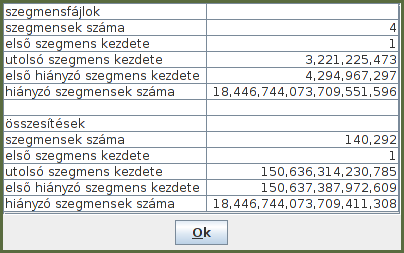
\includegraphics[scale=1]{info.png}
\end{figure}

\subsection{Szegmensek összesítése}

Az adatbázis könyvtárban található új szegmensfájlokat a ''DB összesítés'' gomb megnyomásával, vagy a \texttt{database reaggregate} paranccsal lehet összesíteni.
Minden olyan szegmensfájlról új összesítés készül, amihez még nem tartozott összesítés, vagy a szegmensfájl újabb, mint ami alapján a már meglévő összesítés készült.
Az adatbázisban már meglévő, többi szegmenshez tartozó statisztika nem vész el.

\begin{lstlisting}[language=bash]
scripts$ ./database reaggregate
100.0%
\end{lstlisting}

\subsection{Összesítőfájlok összefésülése}

Lehetőség van egy másik adatbázisból statisztikák átvételére is.
Erre több gépen párhuzamosan szitálva lehet szükség.
Az összefésülést a grafikus felületen a ''DB import'' megnyomása után egy file kiválasztásával lehet indítani.
Parancssorból a \texttt{dabatase import aggregates} \textit{fájlnév} parancs kiadásával.
A megadott fájlból azokat a szegmenseket veszi át a program, amik vagy nincsenek még meg az adatbázisban, vagy megvannak, de az importált statisztikák utolsó módosítási ideje nagyobb az adatbázisban lévőnél.

\begin{lstlisting}[language=bash]
scripts$ ./database import aggregates /valahol/egy/masik/aggregates
100.0%
\end{lstlisting}

\section{Szitatáblák ellenőrzése}

A \texttt{generator} program teszteléséhez a grafikus program képes a szegmensfájlok ellenőrzésére.
Ehhez a \texttt{gui} újra előállítja az ellenőrzött szegmensfájlokat, és azokat összeveti.
Az ellenőrzőszegmensek előállításához az egyszerű szegmentált eratoszthenészi szitát, vagy ez erős pszeudoprím tesztet lehet választani.

A pszeudoprím teszt a szegmens minden számáról egyesével dönti el, hogy az prím-e.
A pszeudoprím teszt rendkívül lassú, a célja, hogy Eratoszthenész szitájához képest egy alapvetően más módszer is rendelkezésre álljon az ellenőrzéshez.

A grafikus felületen a ''Szegmensfájlok ellenőrzése'' gomb megnyomása után lehet kiválasztani a szitálni kívánt szegmenseket, és a referencia előállításának módszerét, majd az ''Ellenőrzés'' gombbal lehet megkezdeni a tényleges folyamatot.

Az ellenőrzést parancssorból is lehet futtatni a \texttt{check-segments} szkripttel.
A szkript első paraméterében a referencia módszerét várja, ami lehet \texttt{sieve}, vagy \texttt{test}, a paraméterek maradéka az ellenőrizendő szegmensek kezdőszáma kell legyen.
Ha egy kezdőszám sincs megadva, akkor a program az adatbázis könyvtárban található összes szegmensfájlt ellenőrzi.

\begin{lstlisting}[language=bash]
scripts$ ./check-segments sieve
100.0%: A szegmensek helyesek.             

scripts$ ./check-segments sieve 0x1 0xc0000001
100.0%: A szegmensek helyesek.             

scripts$ ./check-segments test 0x1
100.0%: A szegmensek helyesek.             

\end{lstlisting}

Az ellenőrzőszegmens szitával történő előállításához szükséges, hogy az \texttt{init} program által előállított négy darab szegmensfájlt tartalmazza az adatbáziskönyvtár.
Az $1$-től kezdődő szegmens kivételével az ellenőrző szegmens előállításához a szita az inicializálásához a prímszámokat innen olvassa fel.

\section{Sziták ellenőrzése}
\label{sec:szitak-ellenorzese}
%%% EMIL: az előző fejezet szatatáblák ellenőrzése volt... ami nagyon hasonlít ehhez a fejezethez... mi a különbség?
%%% P: 1-2 olvasáskörig megfontolom, hogy a "sziták"-at át lehetne nevezve, "a versenyló sziták"- szerű kifejezésre


A sziták futási idejének összehasonlításához írt szitákat is lehet ellenőrizni, az általuk előállított szitatáblák ellenőrzésével.
Az összehasonlításhoz a szegmensek ellenőrzésénél használt egyszerű szegmentált szita a referencia.

A program grafikus felületén a ''Sziták ellenőrzése'' lehetőséget választva ki kell választani az ellenőrizendő szitát, és az ellenőrizni kívánt intervallum kezdő és végző számát.
A folyamat az ''Ellenőrzés'' gomb megnyomásával indítható.

Parancssorból is ellenőrizhetőek a sziták a \texttt{check-sieve} szkripttel.
A szkript 3 paramétere a szita neve, és az intervallum kezdő-, és végszáma.
Az ellenőrizhető sziták nevei:
\begin{itemize}
\item \texttt{atkin}: Atkin szitája\cite{atkin}
\item \texttt{cols}: Cache Optimalizált Lineáris Szita\cite{cols}
\item \texttt{eratosthenes-segmented}: Eratoszthenész szitájának szegmentált változata
\item \texttt{bin-heap} és \texttt{bin-heap-inplace}: Eratoszthenész szitája bináris kupaccal,
	a \texttt{bin-heap-inplace} a kupac javítását helyben végzi
\item \texttt{buckets}, \texttt{buckets-}$n$, \texttt{buckets-simple}: Eratoszthenész szitája, edénysorral
	A \texttt{buckets-simple} nem szegmentált, a \texttt{buckets}, és a \texttt{buckets-}$n$ szegmentált.
	A \texttt{buckets-}$n$-ben az $n$ helyére 1-től 8-ig a számrendszer bitjeit lehet megadni,
	pl. \texttt{buckets-3} 8-as számrendszerben számol
\item \texttt{trial-division}: próbaosztás
\end{itemize}

A \pageref{sec:szitak} oldalon található ''Sziták'' szakaszban található ezeknek a szitáknak a részletesebb leírása.

A sziták nevei listázhatóak a \texttt{list-sieves} szkripttel, a \texttt{describe-sieves} szkript rövid leírást is ad.

\begin{lstlisting}[language=bash]
scripts$ ./check-sieve buckets-3 3000000000001 3010000000001
100.0%: A szita helyes.
\end{lstlisting}

Ha a kezdőszám nagyobb, mint 1, az ellenőrzéshez ilyenkor is szükséges, hogy a négy darab kezdő szegmensfájlt tartalmazza az adatbáziskönyvtár.

\begin{figure}[h]
\caption{Szita ellenőrzése}
\centering
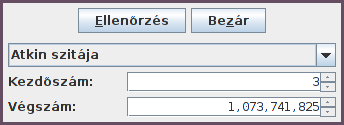
\includegraphics[scale=1]{check-sieve.png}
\end{figure}

\section{Minta megjelenítése}

A \texttt{gui} program a grafikus felületén képes mintákat Descartes-féle koordináta rendszerben ábrázolni, a mintákat függvényekkel közelíteni, és ezeket a függvényeket a mintával együtt ábrázolni.
A program a közelítések négyzetes hibáját is kiszámítja a mintához képest.
A program egyváltozós, egyértékű mintákat kezel, azok között is a természetes számokhoz valós számokat rendelőket.
A minta akár külső forrásból is származhat.

A grafikonábrázoló részt a \texttt{gui-graph} szkripttel lehet indítani. A \texttt{gui} szkripttel indítva, majd a ''Grafikon'' gomb megnyomásával is meg lehet nyitni ezt az ablakot.

Az ablak bal oldalán jelennek meg a betöltött minták és közelítő függvények grafikonjai.
Minta és függvény hozzáadása után a grafikon megjelenített részét a program úgy választja meg, hogy minden minta összes pontja ebbe a nézetbe essen.
A nézet a grafikon feletti gombokkal, vagy egérrel mozgatható, nagyítható, vagy kicsinyíthető.
Az ''Auto.nézet'' gombbal a nézet a minták teljes terjedelmére visszaállítható.

Az ablak jobb oldala a betöltött minták kezelésére szolgál.
A felső harmada az összes betöltött mintát mutatja.
Az ablak jobb oldalának alsó két harmadában az itt kiválasztott minta részletei látszódnak.

\begin{figure}[h]
\caption{Minta megjelenítése}
\centering
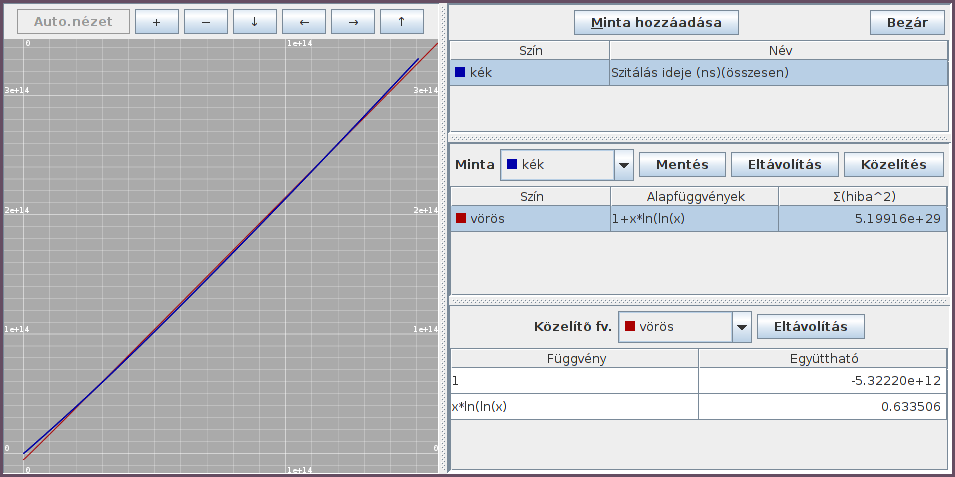
\includegraphics[scale=0.5]{graph.png}
\end{figure}

\subsection{Minta hozzáadása}

A ''Minta hozzáadásánál'' három adatforrásból lehet választani.
A ''Fájl betöltésével'' CSV fájl olvasható be. A fájl formátuma megengedő, az első oszlopot $x$, a második oszlopot $y$ értékeknek próbálja értelmezni, a fel nem ismert sorokat eldobja.
Ha az első sor első oszlopában \texttt{BARS} szerepel, akkor a program a mintát vonaldiagram helyett oszlopdiagramként fogja ábrázolni.

A ''Prímstatisztikák'' a \texttt{generator} kimeneteléből összesített statisztikák. Ezeket a \texttt{gui} program az adatbáziskönyvtárban keresi.
A program a szegmensstatisztikák hiánytalan kezdőszeletét veszi csak figyelembe.
A statisztikáknak három csoportja van.
\begin{itemize}
\item A prímek száma, és néhány kiemelt alakú prím száma minden szegmens végén.
Ide tartozik a prímszámtétel becslése, és a becslés abszolút és relatív hibája is.

\item A prímhézagok statisztikái a szegmensek teljes kezdőszeletére vonatkoznak, az értékek az első szegmenstől a kezdőszelet végéig összesített statisztikából származnak.
A prímhézagok statisztikái az előfordult hézagok gyakorisága, első előfordulása, jósága, valamint a legnagyobb prímhézag adott számig.

\item Ezeken kívül a szegmensek szitálásának ideje is betölthető.
A szegmensenkénti idő minden szegmens végéhez annak a szegmensnek a szitálásának idejét rendeli.
Az összesített idő a szegmensek végéig az összes megelőző szegmens szitálásának idejét adja össze.
\end{itemize}

A minták harmadik forrása a programba épített sziták futási idejének mérése.
Ehhez meg kell adni a szitát, a szitált intervallum elejét és végét, a szita belső szegmensméretét, a generálandó mintaelemek számát, a mérések számát, a mértéket, és hogy az eredményt összesítse-e.

\begin{figure}[h]
\caption{Szita futási idejének mérése}
\centering
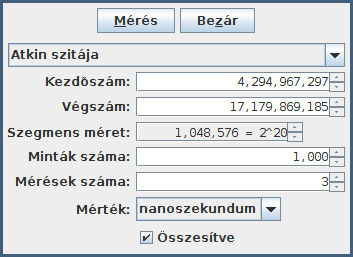
\includegraphics[scale=1.0]{measure.png}
\end{figure}

A sziták listája ugyanaz, mint a sziták ellenőrzősénél.
A mintákat a program a szitált intervallumon egyenletesen osztja el a megadott méretű szegmensek határainál.
A teljes szitálást annyiszor végzi el, amennyi a mérések számában meg volt adva, és az eredményt átlagolja.
Összesítést kiválasztva a mintaelemek értéke a szitált intervallum elejétől az adott számig szitálás teljes ideje, különben az előző minta helyétől.
A mérték szabályozza, hogy a tényleges eltelt időt mérje a program nanoszekundumokban, vagy az elvégzett műveletek számát.

\subsection{Minta közelítése}

Az ablak jobb oldalának középső harmadában a kiválasztott minta részletei látszódnak.
Itt változtatható meg a minta ábrázolásához használt szín, távolítható el a minta, vagy menthető CSV fájlba.

A táblázat a minta közelítéseit mutatja, itt olvashatóak le a közelítés komponensfüggvényei, és a közelítés hibája.
A ''Közelítés'' gombbal lehet új közelítést hozzáadni az ábrázoláshoz.
A közelítéshez a lineáris legkisebb négyzetek módszerét használja a program, ehhez a lineáris kombináció elemi függvényeit meg kell adni.
A függvények kiválaszthatóak az előre megadott listából, vagy JavaScript nyelven is megadhatóak.
A közelítéshez csak olyan függvények használhatóak, amik a minta minden pontjában értelmezve vannak.

\begin{figure}[H]
\caption{A közelítés elemi függvényeinek megadása}
\centering
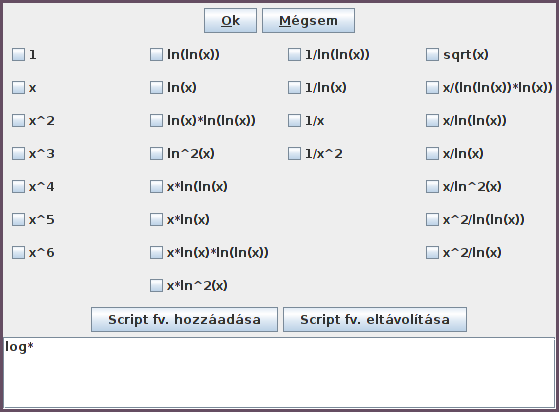
\includegraphics[scale=0.75]{functions}
\end{figure}

JavaScript függvényhez meg kell adni a függvény nevét és forráskódját.
A forráskódban a függvény argumentumára az $x$ változóval lehet hivatkozni, és a szkript utolsó kifejezésének értéke lesz a függvény értéke $x$-ben.
Pl. az $x \mapsto \frac{\ln{x}}{x}$ hozzárendelés forráskódja:

\begin{lstlisting}[basicstyle=\small, language=Java]
Math.log(x)/x
\end{lstlisting}

A szkriptben használható változó, és a szokásos vezérlőutasítások.
Pl. az iterált logaritmus egy megadása:
\begin{lstlisting}[basicstyle=\small, language=Java,morekeywords=var]
var y=0;
while (1<x) {
  x=Math.log(x);
  ++y;
}
y
\end{lstlisting}

Az így megadott függvények visszatérési értéke mindig \texttt{double} típusú kell legyen,
és a függvény azokban a pontokban értelmezett, ahol ez az érték véges.

Egy kiválasztott közelítés részletei az ablak jobb alsó sarkában látszódnak, itt megváltoztatható a közelítéshez rendelt szín, és eltávolítható a közelítés.
A táblázat a közelítéshez kiválasztott függvények együtthatóit mutatja a lineáris kombinációban.

A legkisebb négyzetek módszerének feladata röviden leírható.
Ha az $n$ elemű minta
\begin{align*}
(x_1, y_1), (x_2, y_2), \ldots, (x_n, y_n) (x_i \in \mathbb{N}, y_i \in \mathbb{R})
\end{align*}
és a közelítéshez kiválasztott $m$ függvény
\begin{align*}
f_1, f_2, ..., f_m (f_i:\mathbb{R} \mapsto \mathbb{R})
\end{align*}
akkor a legkisebb négyzetek módszere keresi azokat a
\begin{align*}
c_1, c_2, ..., c_m (c_i \in \mathbb{R})
\end{align*}
skalárokat, hogy az
\begin{align*}
f(x)=\sum_{i=1}^m c_i f_i(x) (x \in \mathbb{R})
\end{align*}
közelítő függvény és a minta eltérése minimális
legyen a
\begin{align*}
\sum_{i=1}^{n} (f(x_i)-y_i)^2
\end{align*}
négyzetes eltérés összeg szerint.

A program ezt az eltérés összeget jeleníti meg a közelítés hibájaként, valamint a $c_i$ skalárok a közelítés elemi függvényeinek együtthatói.

\section{Sziták mérése szkriptekkel}

A sziták futási idejének mintáit parancssorból is elő lehet állítani.
Ilyenkor az eredményt, megjelenítés helyett, a megadott fájlba írja a \texttt{gui} program, ami később a grafikus felületen betölthető.
A méréseket a \texttt{measure-sieve} szkripttel lehet elvégezni, paraméterként meg kell adni ebben a sorrendben:
\begin{itemize}
\item a szita nevét, ezek ugyan azok lehetnek, mint a \pageref{sec:szitak-ellenorzese} oldalon a ''Sziták ellenőrzése'' szakaszban
\item a számot, ahol a szitálás kezdődik, ez páratlan szám kell legyen
\item a szitálás végét, ez páratlan szám kell legyen
\item a szegmensek méretét
\item a mérések számát
\item a minták számát
\item hogy időt (\texttt{nanosecs}), vagy műveleteket (\texttt{operations}) mérjen
\item összesítse az időket (\texttt{sum}), vagy szegmensenként külön számolja (\texttt{segment})
\item a fájlt, ahova az eredményt mentse CSV-ben
\end{itemize}

Ha a kezdőszám nagyobb, mint 1, akkor az adatbáziskönyvtárnak tartalmaznia kell az \texttt{init} program generálta első négy szegmenst.

Lehetőség van a mérték és az összesítés mind a négy kombinációját egy méréssel előállítani, ehhez mind a négy kimeneti fájl meg kell adni külön.

\begin{lstlisting}[language=bash]
scripts$ ./measure-sieve buckets-3 1 0x10000001 0x10000 3 1000 nanosecs sum out1.csv
100.0%
scripts$ ./measure-sieve buckets-3 1 0x10000001 0x10000 3 1000 operations segment out2.csv
100.0%
scripts$ ./measure-sieve buckets-3 1 0x10000001 0x10000 3 1000
seg-ns.csv seg-ops.csv sum-ns.csv sum-ops.csv
100.0%
\end{lstlisting}

A mérések megkönnyítéséhez a \texttt{measure-sieves} szkript az összes szitát megméri, és az eredményt a \texttt{samples} könyvtárba menti.
A \texttt{samples} könyvtárban a mérési eredmények 4 külön könyvtárban szegmensenként/összesítve, és idő/művelet szerinti bontásban vannak.
Ezekben a könyvtárakban 2 fajta mérés eredményei vannak.
Az \texttt{atkin} könyvtárban Atkin szitájának sebessége van megmérve különböző szegmensméretek esetén.
Azokban könyvtárakban, amiknek a neve \texttt{speed}-del kezdődik, az összes szita sebességének mérése található, $2^{20}$ szegmensmérettel.
A könyvtárak nevében a szám a szitálás kezdetét adja meg, a \texttt{speed}$n$ nevű könyvtárban a mérések $2^n+1$-től kezdődnek.
A lassabb szitákat csak kisebb nagyságrendekre méri meg a szkript, ezek futási ideje hamar túl naggyá válik.

A \texttt{measure-generator} szkript a \texttt{generator} program sebességét méri meg.
A mérés 3 paramétert variál, a szitálás kezdetének nagyságrendjét, a szegmensméretet, és az edénysor számrendszerét.
Az eredményt a \texttt{samples/measure-generator.csv} fájlba menti.
Ez nem használható a program mintamegjelenítésével, mert az egy változós mintákkal dolgozik.
Ennek a mérésnek a célja az, hogy a \texttt{generator} program paramétereit egy konkrét számítógéphez lehessen igazítani.
A szkript 16 egymás utáni szegmensfájlt szitál,
\begin{itemize}
\item a szitálás kezdetét $2^{33}$-től $2^{63}$-ig változtatja, a kitevőt hármasával növelve
\item a szegmensek méretét $2^{16}$-tól $2^{24}$-ig, a kitevőt egyesével növelve
\item és a számrendszert $2^1$-től $2^8$-ig, szintén a kitevőt egyesével növelve.
\end{itemize}

%%% Local Variables:
%%% mode: latex
%%% TeX-master: "szakdolgozat"
%%% End:


\chapter{Fejlesztői dokumentáció}

\section{A feladat leírása}

A program feladata, hogy lehetővé tegye prímsziták futási idejének összehasonlítását.
A prímsziták az egész számok egy intervallumán
minden számról eldöntik, hogy a szám prím, vagy összetett.
A program keretet ad, hogy azonos paraméterekkel lehessen a sziták futási idejét mérni,
és egyszerű, egymáshoz hasonlóan optimalizált szitákat implementál,
hogy a futási időket a fő algoritmusok határozzák meg, mivel a szitálást felgyorsító
egyes ötletek nem minden szitán alkalmazhatóak.
A futási időt eltelt időben, és összeszámolt műveletekben is méri.

A szitákat szegmentáltan valósítja meg,
a szegmensek mérete, és a szitálandó intervallum
kezdete és vége szabályozható. A megvalósított sziták:
\begin{itemize}
\item Atkin szitája
\item Eratoszthenész szitája
\begin{itemize}
\item egyszerű tömbbel
\item bináris kupaccal
\item edényekkel
\item monoton edénysorral
\end{itemize}
\end{itemize}

A programnak grafikusan ábrázolja a futási időket, és lehetőséget ad
ezek közelítésére függvényekkel. A közelítéshez a legkisebb négyzetek módszerét használja,
és a közelítés elemi függvényei megválaszthatóak.
A program megjeleníti a közelítések négyzetes eltérését is a mintához képest.
Elemi függvény meg lehet adni JavaScript nyelven is.

A grafikus ábrázolás képes külső forrásokból származó minták megjelenítésére és közelítésére is.

A minták és függvények ábrázolása interaktív, az éppen megjelenített
intervallum elhelyezkedése és mérete megválasztható.
Egyszerre több mintha is megjeleníthető,
és minden mintához egyszerre több közelítő függvény is tartozhat.

A prímszámok statisztikáinak megjelenítéséhez
elő tudja állítani ezeket a statisztikákat nagyobb intervallumokon is.
Ehhez ad egy szitát, ami hatékonyan képes $2^{64}$-ig szitálni,
és ennek az eredményét összesíteni. Az előállítható statisztikák
adott $n$-ig szitálva:
\begin{itemize}
\item a prímek száma
\item a $4\mathbb{Z}+1, 4\mathbb{Z}+3, 6\mathbb{Z}+1, 12\mathbb{Z}+11$
	alakú prímek száma
\item ikerprímek számát
\item az előforduló prímhézagok első előfordulásának helye
\item a prímhézagok előfordulásának száma
\item a szitálásra fordított idő
\end{itemize}

A prímek számát, és a szitálás idejét az intervallum belsejében is több ponton elkészíti.

A sziták sebességének mérését, és a statisztikák előállítását
parancssorból is el tudja végezni, hogy szkriptekkel ez automatizálható legyen.
A statisztikák előállításának folyamata
bármikor adatvesztés leállítható, és később folytatható.

%%% EMIL: kb eddig olvastam, a többin csak átfutott a szemem... majd mindjárt írok levelet.

\pagebreak
\section{A program komponensei}

\begin{figure}[h]
\centering
\caption{A program adatáramlás diagramja}
\begin{tikzpicture}[framed]
\draw (0, 0) node[rectangle,draw](db) {Adatbázis};

\draw (-1, 1) node[rectangle,rounded corners,,draw](init) {init};
\draw (1, 1) node[rectangle,rounded corners,,draw](generator) {generator};
\draw (4, 1) node[rectangle,rounded corners,,draw](aggregate) {Összesítés};
\draw (4, 0) node[rectangle,draw](info) {Info};

\draw (-4, 1) node[rectangle,rounded corners,draw](check-segment) {Szegmens ellenőrzése};
\draw (-4, 0) node[rectangle,rounded corners,,draw](reference-sieve) {Referencia szita};
\draw (-4, -1) node[rectangle,rounded corners,,draw](check-sieve) {Szita ellenőrzése};
\draw (0, -1) node[rectangle,rounded corners,,draw](sieves) {Sziták};

\draw (4, -1) node[rectangle,draw](view) {Megjelenítés};
\draw (4, -2) node[rectangle,rounded corners,,draw](approximate) {Minta közelítése};

\draw[<->, thick] (db) -- (aggregate);
\draw[->, thick] (db) -- (check-segment);
\draw[<->, thick] (db) -- (generator);
\draw[->, thick] (db) -- (info);
\draw[->, thick] (db) -- (reference-sieve);
\draw[->, thick] (db) -- (sieves);
\draw[->, thick] (db) -- (view);
\draw[->, thick] (init) -- (db);
\draw[->, thick] (reference-sieve) -- (check-segment);
\draw[->, thick] (reference-sieve) -- (check-sieve);
\draw[->, thick] (sieves) -- (check-sieve);
\draw[->, thick] (sieves) -- (view);
\draw[<->, thick] (view) -- (approximate);

\draw[dashed, rounded corners] (-6.2, 0) -- (-6.2, 1.5) -- (-1.7, 1.5) -- (-1.7, -0.5) -- (2.7, -0.5) -- (2.7, 1.5) -- (5.8, 1.5) -- (5.8, -2.5) -- (-6.2, -2.5) -- (-6.2, 0);
\draw (-5.7, -2.2) node[]{gui};
\draw[dashed, rounded corners] (-6.2, -1.8) -- (-5.1, -1.8) -- (-5.1, -2.5);
\end{tikzpicture}
\end{figure}

A program az adatbáziskönyvtárban tárolja az átszitált szegmensek tábláit, és az ezekből készült statisztikákat.
A szegmensfájlokban egy $2^{30}$ hosszú intervallum minden páratlan számához hozzá van rendelve, hogy az az szám összetett vagy prím, és minden szegmens kezdő száma kongruens $1 (mod\ 2^{30})$.

Az első négy szegmenst az init program készíti el, így ezek $2^{32}$-ig tartalmazzák a prímszámokat.
A program többi szitája ezek alapján inicializálja magát, ha $3$-nál nagyobb számtól kell a szitálást elkezdeni.
Ez a négy fájl bármikor újragenerálható, de ezeket érdemes a futások között megtartani.

A generátor egy optimalizált szita, $2^{32}$-től $2^{64}-2^{34}$-ig képes szitálni, mindig egész szegmenseket, és az eredményt az adatbáziskönyvtárba menti.
Ezekre a szegmensfájlokra összesítés és ellenőrzés után többet nincs már szükség.
A szitálást tetszőleges szegmenstől lehet kezdeni a megengedett tartományon belül, nem szükséges sorban végigmenni a számokon.
Az utolsó $2^{34}$ szám kihagyása egyszerű optimalizáció, így a programban az éppen szitált szám változója sosem csordul túl.

Az init és a generator csak konzol módban futtatható.
A program többi része a gui nevű Java program része, de az automatizáláshoz az adatbázissal kapcsolatos műveletei parancssorból is elérhetőek, ezek az adatbázis információ lekérése, az új szegmensfájlok ellenőrzése, és összesítése, és az összesítőfájlok összefésülése.
Az időigényessége miatt a futási idő összehasonlításához implementált sziták ellenőrzése is futtatható grafikus felületen, és parancssorból is.

Az adatbázis információ kilistázza a szegmensfájlok számát, az összesített szegmensfájlok számát, ezen szegmensek intervallumának kezdetét és végét, a még nem összesített szegmensfájlok számát.
Ezek alapján eldönthető, szitálást vagy az összesítést hogyan kell folytatni, hogy a teljes $2^{64}$-ig intervallum statisztikái elkészüljenek.

A szegmensfájlok ellenőrizhetőek, ehhez egy, a generator-tól különböző eratosthenészi szita, vagy az erős pszeudo-prímteszt\cite{pseudoprime}\cite{pseudoprimebase} előállítja a szegmens ellenőrzött részét, és a program a kettőt összehasonlítja.
A szita lényegesen lassabb, mint a generator, és a pszeudo-prímteszt időigénye miatt intervallumok szitálásra nem alkalmas, a szegmensfájlok ellenőrzése alapvetően a generator helyességének
tesztelésére való, minden összesített szegmens ellenőrzése megtöbbszörözné a szükséges időt.

Az összesítő az adatbáziskönyvtárban található szegmensfájlok statisztikáit készíti el, és ezeket a szegmensstatisztikákat szintén az adatbázisban tárolja.
A szegmensstatisztikák alapján a végső statisztikákat közvetlenül a megjelenítés előtt készíti el az összesítő.
Az összesítéshez sem szükséges, hogy a szegmensek sorban kerüljenek összesítésre, így akár több gépen párhuzamosan is lehetne szitálni, összesíteni, majd az eredményt összefésülni.

A program része több, különböző algoritmusú prímszita.
Ezeknek az eredménye ellenőrizhető a szegmensfájlok ellenőrzéséhez használt szitával, szintén a sziták helyességének teszteléséhez.
A feladat része, hogy ezeknek a szitáknak a futási idejét össze lehessen hasonlítani, ezért mindegyik szita néhány jól meghatározott ötlet egyszerű megvalósítása optimalizálások nélkül.
Mindegyik szita szegmentált, a szitálást fix hosszúságú intervallumokon végzi, bármelyik szegmenstől képes kezdeni a szitálást, és egy szegmens szitálása után további előkészület nélkül képes szitálni a következő szegmenst, így egyetlen menetben akár több szegmenshez tartozó futási idő is megmérhető, nem szükséges minden mintavételi pontig a teljes szitálást elvégezni.

A minták közelítése alapfüggvények lineáris kombinációjával történik, a legkisebb négyzetek módszerét használva.

A program a mintákat és közelítő függvényeket Descartes-féle koordináta rendszerben jeleníti meg, ehhez a mintákat és a függvényeket mintavételezi az x tengely kiválasztott szakaszának pixelenkénti felosztása szerint.

\section{Az adatbázis}

A program adatbázisa két fajta adatot tárol, a szitált szegmenseket, azaz a szitatábla bitvektorait, és a szegmensek összesítéseit.
Mindkettő a szegmens első számával van azonosítva, a szegmens hossza mindig $2^{30}$ szám, és az $n \in \mathbb{N}$ megengedett kezdő szám, ha $n < 2^{64}-2^{34}$ és $n \equiv 1 \pmod{2^{30}}$.
Minden szegmens egy külön fájl az adatbázis könyvtárában, és az összes szegmensstatisztika egy fájlban van.

Az init program az első 4 szegmensfájlt írja, a generator az első 4 szegmensfájlt olvassa, és az összes többi szegmensfájlt írja, a gui az összes szegmensfájlt olvassa, és egyiket se írja, és szegmensstatisztika fájlt csak a gui használja.

Egy szegmensfájlok nevei ''primes.'' előtaggal kel kezdődjön, és a pontosan 16 hexadecimális számjegy kell kövesse, ami a szegmens által leírt első szám.
A fájl bináris fájl, a legkisebb helyiértékű bájt elöl.
A tartalma:
\begin{itemize}
\item a szegmens elejével kezdve $2^{29}$ egymást követő páratlan szám bitvektora.
	
Ez $2^{26}$ byte, legkisebb helyiértékű byte elöl sorrendben, minden bit egy páratlan szám összetettségét írja le.
Ha a bit $1$, akkor a szám összetett, ha $0$, akkor a szám prím.
Ha $s$ a szegmens intervallumának kezdete, akkor az $0.$ bájt $0.$ bitje $s$-t írja le, a $0.$ bájt $1.$ bitje $s+2$-t, a $k.$ bájt $l.$ bitje $s+16k+2l$-t.
	
\item a szegmens kezdete, 8 bájt, egész
\item a szegmens szitálására való felkészülés ideje, 8 bájt, egész, nanoszekundumokban
\item a szegmens szitálásának ideje, 8 bájt, egész, nanoszekundumokban
\end{itemize}

Ahhoz, hogy az init és a generator program bármikor leállítható legyen szegmensfájl írása közben, a szegmenst először egy ideiglenes fájlba írja, és ha ez hiba nélkül megtörtént, akkor az ideglenes fájlt átnevezi a megfelelő névre.
Mivel az ideiglenes fájl ugyanabba a könyvtárba kerül, mint ahova a szegmensfájl is, így feltételezhető, hogy helyi meghajtón az átnevezés már atomi művelet.

Ez az eljárás az átnevezés előtt nem győződik meg arról, hogy az ideiglenes fájl minden része
kiíródott a háttértárra, így ez csak a program leállíthatóságát garantálja, a számítógép váratlan leállása esetén érdemes azokat a szegmensfájlokat letörölni, amikről feltételezhető, hogy nem volt ideje a számítógépnek minden részét kiírnia a tényleges tárolóra.

A szegmensstatisztikák az ''aggregates'' fájlban vannak. A szegmensek a fájlban a kezdőszámok sorrendjében követik egymást, egy szegmensnek legfeljebb egy statisztikája lehet.
A fájl bináris, a legnagyobb helyiértékű bájt elöl. A fájl fejléce:
\begin{itemize}
\item formátum azonosító: 0xd1d1b0b0, 4 bájt
\item verziószám: 1, 4 bájt.
\end{itemize}
Ezután minden statisztika egy változó méretű blokkban van tárolva, a fájl végéig. Minden block két részből áll, az első 4 bájt a második rész mérete bájtokban. Ez a második rész a szegmensstatisztika. A statisztika gzip-pel tömörített, kitömörítve bináris adat, a legnagyobb helyiértékű bájt elöl, aminek a formátuma:
\begin{itemize}
\item a szegmens összesítésének futási ideje, 8 bájt, nanoszekundumokban
\item a szegmens szitálásának inicializálásának ideje, 8 bájt, nanoszekundumokban
\item az összesített szegmensfájl utolsó módosításának ideje, 8 bátj, milliszekundumokban, 1970.1.1. 00:00:00-tól
\item a szegmensben található legnagyobb prím, 8 bájt
\item a szegmensben található legkisebb prím, 8 bájt
\item a $12\mathbb{Z}+11$ alakú prímek száma a szegmensben
\item a $4\mathbb{Z}+1$ alakú prímek száma a szegmensben
\item a $4\mathbb{Z}+3$ alakú prímek száma a szegmensben
\item a $6\mathbb{Z}+1$ alakú prímek száma a szegmensben
\item a szegmensben előforduló prímhézagok számát, 4 bájt. ahány prímhézag előfordult, annyiszor ismétlődik a következő három mező
\begin{itemize}
\item a prímhézag nagysága, 8 bájt
\item a prímhézag előfordulásainak száma, 8 bájt
\item a prímhézag első előfordulása, 8 bájt
\end{itemize}
\item a szegmens sorszáma, 8 bájt
\item a szegmens vége, 8 bájt
\item a szegmens kezdete, 8 bájt
\item a szegmens szitálására fordított idő, 8 bájt, nanoszekundumokban.
\end{itemize}

Az összesítésfájl írása a szegmensfájl írásához hasonló.
Egy ideiglenes fájlba írása után a program megvárja, hogy a fájl tartalma a háttértárolóra íródjon, majd az ideiglenes fájlt átnevezi a megfelelő névre.
Az ideiglenes fájl kiírásának megvárásával a statisztikafájl váratlan számítógép leállás esetén is visszaállítható.

A fájl formátuma és az új fájl kiírásának algoritmusa lehetővé teszi, hogy a statisztikafájlt egyszerre lehessen sorban felolvasni, és az új eredményt sorban kiírni, úgy, hogy egyszerre csak egy statisztikát kelljen a memóriában tartani.

Az adatbázis nincs védve a párhuzamos írásoktól, és az összesítőfájl egyszerű sorban feldolgozhatósága feltételezi, hogy egy fájl kevés szegmensstatisztikát fog tartalmazni, legfeljebb. kb. $10^6$ szegmensét.

\section{A megvalósítás}

A megoldás 3 programból áll, az init és a generator C nyelven készült el, az összes többi részfeladat a gui nevű Java nyelven írt programban lett megoldva.

\subsection{Init és generator}

Az init és a generator forráskódja a tarball generator könyvtárában van.
A két program egymáshoz nagyon hasonló feladatot lát el, hasonló megoldásokkal.
Mindkettő $2^{30}$ hosszú intervallumokat szitál, és az eredményt szegmensfájlokba írja.
Ehhez mindkettő Eratoszthenés szitáját használja.
Mindkét program ezt az egyetlen feladatot oldja meg, és szkriptekkel automatizált, kötegelt futásra van tervezve.

\subsubsection{Közös rész}

A két program közös kódja a common.h fájl.
Ez a fájl tartalmazza a konstansokat, és az eljárásokat, amik megkönnyítik a POSIX hívások használatát.
A legtöbb ilyen könnyítés a hibák kezelésének elfedése, ami a kötegelt futtatáshoz illeszkedően
a hiba kijelzése utáni azonnali programleállás.
Az I/O műveleteket könnyítik meg a readFully/writeFully
eljárások.

A sziták belső, kis szegmensmérete a
SEGMENT\_SMALL\_SIZE\_BITS\_LOG2 konstanssal
szabályozható, és a measure-generator szkript
kimenete alapján egy adott géphez igazítható.

A szegmensfájlok olvasására és írásara a readSegment() és writeSegment() függvények szolgálnak.

\subsubsection{Init}

Az init program előállítja az első 4 szegmens fájlt, azaz $2^{32}$-ig az összes prímet megkeresi.
Ezzel a többi részprogram már a $2^{32} - 2^{64}$ tartomány tetszőleges részén tud szitálni, anélkül, hogy a szitált szegmenseket a szitálás után végig kéne nézze új prímekért.

A szita egy egyszerű szegmentált eratoszthenészi szita.
A $2^{30}$ hosszú szegmenseket több kisebb, egyenlő szegmensre osztja, és ezeket a kis szegmenseket
egymás után szitálja a prímek listáján végigmenve.
A prímek mellett a következő szitálás helyét is eltárolja, így nem kell minden szegmens szitálásának elején minden prímhez osztással meghatározni, hogy melyik a legkisebb szám a szegmensben, amit az oszt.
Így egy kis szegmensben egy prímre a következő algoritmus fut le.
Ez az algoritmus visszatérő minta a szegmentált szitákban.

\begin{algorithmic}[1]
\State p: \text{a prím}
\State q: \text{a következő szám, amit p oszt}
\State e: \text{a szegmens vége}
\While{q < e}
	\State \Call{Megjelöl}{q}
	\State q = q + 2p
\EndWhile
\end{algorithmic}

A prímek listáját elég $2^{16}$-ig előállítai, ezt a program próbaosztással végzi el.

\subsubsection{Generator}

A generator fő részei hasonlóak az init-hez.
Indulása után felolvassa az összes prímet az első 4 szegmensfájlból, és mindegyik prímhez osztással meghatározza, hogy melyik a legkisebb szám, amit oszt, és legalább akkora, mint legelső
szitálandó szegmens kezdete.
A prímek, és a hozzájuk tartozó következő szitálandó pozíciót tároló adatstruktúra szitálás közben
nem érzékeny azokra az elemekre, amik az éppen szitált szegmensnél nagyobb helyeken szitálnak, így a generator az összes prímet eltárolja $2^{32}$-ig, nem csak a szitálandó tartomány végének négyzetgyökéig, és a prímek első többszörösét is a prím négyzetétől szitálja.

A prímek listájának inicializálása után a nagy szegmenseket az inithez hasonlóan kisebbekre osztja,
és ezeket sorban szitálja a prímek listája alapján.

A prímek listája a generatorban több külön adatszerkezet összessége.
A prímeket a szita inicilizálásánál 3 részre osztja a nagyságuk szerint.
A $64$-nél kisebb prímeket $64$-bit széles bitmintákban tárolja, és ezekkel a mintákkal $64$-bitesével szitálja végig a kis szegmenseket a bitenkénti vagy művelettel.
A 3 és a 11, valamint az 5 és a 7 szorzata kisebb, mint 64, ezeket a párokat egyetlen $64$ bites mintába fejti ki, ezeknek a mintáknak a periódisa 33, és 35.
A többi prím mintájának periódusa a legnagyobb olyan szám, ami 64-nél kisebb, és a prím osztja.

A prímek, amik $64$-nél nagyobbak, de a kis szegmensek hosszánál kisebbek, azaz minden kis szegmensben szitálnak, az init-hez hasonlóan egy egyszerű tömbbe kerülnek, és ugyanúgy szitál ezekkel a program, mint az init-ben.

A kis szegmensek hosszánál nagyobb prímek egy kis szegmensben legfeljebb egyszer szitálnak, és van olyan szegmens, ahol egyszer sem.
A generator ezeket a prímeket egy prioritásos sorban tárolja, amiben az elemek sorrendjét a következő szegmens száma határozza meg, amiben az a prím szitálni fog, a szegmensen belüli sorrendet a sor nem veszi figyelembe.
Ezeknél a nagy prímeknél nem csak a páros többszörösöket ugorja át a szita, hanem a 3-mal és 5-tel osztható többszörösöket is kihagyja.

Az edénysor algoritmusának részletes leírására egy későbbi fejezetben kerül sor.
Az ott leírt távolság függvényt implementálja a bucketIndex függvény a forráskódban.
A számrendszert a BUCKET\_BITS konstans szabályozza.
A sorhoz tartozó edények listája a buckets tömb, ennek minden eleme egy láncolt lista, ahol a listaelemek fix méretű edények.

A program futása alatt a sor elemeinek száma nem változik, de az elemek az edények között mozognak.
A sor legkisebb elemeinek, azaz az aktuális szegmensben szitáló prímek megkereséséhez a lista egyik edényének minden elemét megvizsgálja, ha egy elem az aktuális szegmensben nem szitál, akkor az elemet a sorba visszahelyezi, a távolság függvény szerint már közelebbi edénybe, ha pedig az elem szitál az aktuális szegmensben, akkor elvégzi a szitálást, és az elemet visszateszi a sorba, azon pozíció szerint, ahol a prím legközelebb szitálni fog.

A 2, 3, és 5 többszöröseinek hatékony kihagyásához
a prioritásos sor elemeiben a pozíció mellett el van tárolva,
hogy az a pozíció melyik modulo 30 maradékosztály eleme.
A nyolc szóba jöhető lehetőség közül a PrimePosition.prime mező
felső 3 bitje választ. Ezt a 3 bit információt biztonsággal
lehet itt tárolni, a 64 bit széles változóból a feladat határai
miatt mindig csak az alsó 32 tartalmaz értékes számjegyet.
Ez a 2-3-5 kerék alapú gyorsítás csak a prioritásos sorban
tárolt nagy prímekre van alkalmazva.

\subsection{Gui}

A program Javaban írt része tartalmazza az összes többi funkció megvalósítását, a szegmensfájlok feldolgozását, a különböző szitákat, és a minták megjelenítését.
Ezeknek a funkcióknak a többsége nem interaktív, a felhasználó a paraméterek megadása után a végrehajtást már nem tudja befolyásolni.

A forráskód ennek megfelelően három egymástól jól elkülöníthető részre osztható.
A legalsó szint a program adatszerkezeteit, algoritmusait, és fájlformátumait írja le. 
Erre építenek a felhasználói műveletek megvalósításai.
Mindegyik művelethez tartozik egy eljárásként megvalósított belépési pont,
a programkód legfelső szintje ezeket teszi a felhasználó számára meghívhatóvá, parancssorból és grafikusan is.

A grafikonmegjelenítés az egyetlen ténylegesen interaktív feladat, ennek megoldása a modell-nézet-vezérlő felosztást alkalmazza.

\subsubsection{gui.util}

A csomag néhány közismert algoritmust és adatszerkezetet tartalmaz, valamint az ezekhez szükséges funkcionális interfészek definícióit.
A legtöbbnek létezik könnyen használható sztenderd könyvtári megvalósítása, de ezek referenciatípusokat használnak.
A primitív és referencia típusú értékek közötti rengeteg konverzió három problémát okoz.
Feleslegesen növeli a futási időt, miközben egyetlen számítógépen szitálva $2^{64}$-ig reménytelenül hosszú feladat.
Ezen túl megnöveli a program memóriaigényét.
$2^{32}$-ig kb. $2\cdot10^6$ darab prím van, ha egy szita csak a prím-pozíció párokat egy egyszerű tömbben tárolná, prímenként 4 bájton, pozícionként 8 bájton, akkor ez a tömb kb. $2,4$Gb memóriát foglalna el.
A program a primitív típusokon alapuló konténerekkel képes $3,5$Gb memória használatával futni.
A harmadik probléma az, hogy primitív érték objektummá alakítása szinte mindig új objektum allokálásával jár, ami legtöbbször egy objektum elérhetetlenségéhez is vezet.
A szemétgyűjtő ezzel járó folyamatos háttérmunkája nem csak feleslegesen növeli a futási időt, hanem kiszámíthatatlanságával megnöveli a sziták mért futási idejének zaját.

A PrimitiveList osztály és leszármazottai az ArrayList mintájára szükség szerint növekvő vektorok. Konkrét megvalósítások a double, int, és long primitív típusokra vannak.

A BinarySearch és a QuickSort a bináris keresés és a gyorsrendezés algoritmusát valósítják meg absztrakt módon elért tömb felett. Az elemeket közvetlenül sosem érik el, az összehasonlításokat és a cseréket interfészeken keresztül végzik index alapján.

A BinaryMinHeap egy bináris kupac, mint absztrakt konténerosztály, az elemek típusától függő műveleteket absztrakt metódusként határozza meg.
A műveletek felteszik, hogy az elemek indexelhetőek, mint egy tömbben.
A kupac egy elsőbbségi sor, a sor eleje az absztrakt rendezés szerinti legkisebb elem.

\subsubsection{gui.math}

Ebben a csomagban az osztályok két részre oszthatóak.
Az UnsignedLong a Java long típus előjel nélküli műveleteit valósítja meg.
A Java a 8-as verziótól támogatja a primitív egész típusok előjel nélküli összehasonlítását és osztását, ez az osztály ezekre építve ad néhány segédeljárást.
A pszeudoprím-teszthez a maradékos hatványozás Java támogatás nélkül a kitevő bitjei alapján az ismételt szorzást és négyzetre emelést használja, míg a szorzás ehhez hasonlóan összeadást és kétszerezést. Ezeknek az algoritmusoknak a futási ideje egy-egy szám esetén elfogadható, de intervallumok szitálására nem alkalmas.

A csomag többi osztálya a legkisebb négyzetek módszerének implementációja, és annak segédosztályai.
A Sum double típusú értékek véges összegeit számolja ki.
A double véges pontosságának következménye, hogy nem minden szám reprezentálható double értékként, és többtagú összeg eredménye függhet a tagok összeadásának sorrendjétől, azaz az összeadások sorrendje befolyásolhatja az eredmény hibáját.
A Sum három stratégiát ad az összeadások sorrendjéből származó hiba minimalizálására.
A program használata közben a felhasználó ezek közül nem tud választani, a tesztek alapján legstabilabbnak ítélt elsőbbségi soron alapuló összegzést használja a közelítés.
A legegyszerűbb Sum.Simple egyetlen változót használva a tagokat felsorolásuk sorrendjében adja össze.
A bináris kupacot használó Sum.Priority a tagokat az elsőbbségi sorban gyűjti, majd a végső összeg kiszámításához a sorból, amíg lehet, ismételten kiveszi a két legkisebb abszolút értékű elemet, azokat összeadja, és az eredményt a sorba visszahelyezi. A végeredmény a sorban maradó érték lesz.
A Sum.Array nagyságrend szerinti részösszegeket tart nyílván, új tagot a nagyságrendjéhez tartozó részösszeghez adja hozzá.
A nagyságrend a double érték IEEE 754 szabvány szerinti reprezentációjának kitevője.

A RealFunction interfész valóshoz valóst rendelő függvények reprezentációi.
Egy függvény a helyettesítési értékein kívül az értelmezési tartományáról is információt kell adjon.
A grafikonmegjelenítő az x-tengely egy pixel által lefedett intervallumán akkor jelenít meg értéket, ha az az intervallum az értelmezési tartomány része.
A Functions osztály a beépített elemi függvényeket tartalmazza.
JavaScript-ben függvény a CustomFunction-nel adható meg.
A LinearCombinationFunction már létező függvények lineáris kombinációja.
A mintaközelítés eredménye ilyen típusú.

A Matrix osztályban vannak megadva a valós mátrixok műveletei, mindegyik kétdimenziós double tömbökre.
Az implementált műveletek a legkisebb négyzetek módszeréhez szükségesekre korlátozódnak.
A Gauss-eliminációnál kiválasztható, hogy részleges sorcserére, vagy teljes sor és oszlopcserére kerüljön sor.
A tesztek alapján a teljes csere lényegesen csökkenti a számítás hibáját, a felhasználó részleges sorcserét nem tud választani.

A LeastSquares osztályban lett megvalósítva a legkisebb négyzetek módszere. A csomag eddig felsorolt osztályaival itt lehet megadni a közelítéshez, a mintán kívül, az elemi függvényeket, és a pontosságot szabályozó paramétereket.
A közelítés hibáját is ki lehet ezzel az osztállyal számolni.

\subsubsection{gui.io}

A gui.io csomagban az adatbázis kezelését leíró osztályok vannak.
Az adatbázis funkciók a Database egy objektumán keresztül érhetőek el, ez a common.h-val párhuzamosan definiálja a szegmensfájlok neveit.
A felhasználói műveletek közül az adatbázis információk lekérését, a szegmensfájlok összesítését, és összesítés importálását Database osztály info(), reaggregate(), és importAggreagtes() metódusai
valósítják meg.
A sziták az inicializálásukkor a Database.largePrimes() metódust használva olvassák be az első 4 szegmensfájlból a prímeket.

A Segment osztály példányai szegmensfájlok a memóriában.
Ezek tényleges fájlból olvasott adatokat is tartalmazhatnak, vagy szegmensek és sziták ellenőrzésekor a Java program is generálja.
Ezzel az osztállyal szegmensfájlt csak olvasni lehet, írni nem.

Egy szegmens összesítését a Segment.aggregate() függvény végzi.
Az eredményül kapott Aggregate példány az adatbázis formátumánál leírt szegmensstatisztika tükre.
Az összesítőfájlt az AggregatesReader és AggregatesWriter osztállyal lehet írni és olvasni, mindkét esetben a szegmensek szigorúan növekedő kezdőszámú sorrendben dolgozhatóak fel.
A írás és az olvasás AggregateBlock példányokkal dolgozik, ezek az objektumok a statisztikához való hozzáférés mellett a betömörített bináris adatot jegyzik meg, hogy a statisztika változatlan kiírása esetén ki lehessen hagyni az időigényes betömörítést.

Az szegmensenkénti statisztikák alapján a megjelenítésre szánt mintákat az Aggregates osztály készíti el.
A szegmenseket az összesítésfájl sorrendjében dolgozza fel, az első hiányzó szegmensig. A megjelenített statisztikák legtöbbje egyszerűen összesíthető a szegmensenkénti adatokból. A prímhézagok esetében a szegmenseken átívelő hézag külön odafigyelést igényelnek.

Ez a csomag tartalmazza a CSV fájlok olvasásához és írásához a CSVReader és CSVWriter osztályokat. Mindkettő stream alapon teszi lehetővé a szöveges cellák soronkénti feldolgozását.

\subsubsection{gui.sieve}

Ebben a csomagban, és a gui.sieve.eratosthenes alcsomagjában, a futási idők méréséhez implementált sziták vannak.

\begin{figure}[H]
\centering
\caption{A sziták osztály diagramja}
\begin{tikzpicture}[framed]

\umlclass[x=0.5, y=0, type=abstract]{OperationCounter}{}{
+add() \\
+get()::long \\
+increment() \\
+reset()}

\umlclass[x=5.5, y=-0.3, type=abstract]{SieveTable}{}
{+clear(prime) \\
+flip(number) \\
+isPrime(number)::boolean \\
+setComposite(number) \\
+setPrime(number)}

\umlclass[x=10, y=1]{LongTable}{}{}
\umlclass[x=10, y=-1]{Segment}{}{}
\umlclass[x=0, y=-4, type=abstract]{Sieve}{}{+reset(start) \\ +sieve()}
\umlclass[x=0, y=-7, type=abstract]{SegmentedSieve}{}{}
\umlclass[x=0, y=-9.5, type=abstract]{EratosthenesianSieve}{}{}
\umlclass[x=4, y=-4]{TrialDivision}{}{}
\umlclass[x=4, y=-6]{SieveOfAtkin}{}{}
\umlclass[x=9, y=-6]{SieveOfEratosthenes}{}{}
\umlclass[x=8, y=-8]{QueueSieve}{}{}
\umlclass[x=7, y=-10]{CacheOptimizedLinearSieve}{}{}
\umlclass[x=6, y=-12]{SimpleBucketSieve}{}{}
\umlclass[x=1, y=-12, type=abstract]{BucketSieve}{}{}
\umlclass[x=1, y=-14]{Bucket1Sieve}{}{}
\umlclass[x=5, y=-14]{BucketNSieve}{}{}

\umlinherit{LongTable}{SieveTable}
\umlinherit{Segment}{SieveTable}
\umluniassoc{Sieve}{SieveTable}
\umluniassoc{Sieve}{OperationCounter}
\umlinherit{SegmentedSieve}{Sieve}
\umlinherit{TrialDivision}{Sieve}
\umlinherit{EratosthenesianSieve}{SegmentedSieve}
\umlinherit{SieveOfAtkin}{SegmentedSieve}
\umlinherit{BucketSieve}{EratosthenesianSieve}
\umlinherit{SieveOfEratosthenes}{EratosthenesianSieve}
\umlinherit{QueueSieve}{EratosthenesianSieve}
\umlinherit{CacheOptimizedLinearSieve}{EratosthenesianSieve}
\umlinherit{SimpleBucketSieve}{EratosthenesianSieve}
\umlinherit{Bucket1Sieve}{BucketSieve}
\umlinherit{BucketNSieve}{BucketSieve}
\end{tikzpicture}
\end{figure}

A sziták a Sieve osztály leszármazottai.
A példányaitól elvárás, hogy
\begin{itemize}
\item a szitálást szegmensenként végezzék
\item a szitatábla bitvektorát csak korlátozottan éri el
\begin{itemize}
\item csak az éppen szitált szegmensbe eső számokat éri el
\item páros számot sose ér el
\item legfeljebb $2^{32}-1$-ig olvassa vissza a szitálás eredményét
\end{itemize}
\item a szegmens mérete szabályozható, a lehetséges értékek a kettő hatványai $2^8$-tól $2^{30}$-ig 
\item bármikor újra lehessen inicializálni a szitát egy szegmens kezdetéhez úgy, hogy onnantól már további felkészülési idő nélkül több egymás utáni szegmenst tud szitálni
\item az OperationCounter osztály segítségével számon tartja a szitálás műveletigényét.
\end{itemize}

A SieveTable osztály Segment implementációja az adatbázisnál is használt szegmensfájl, szita ellenőrzésekor ez a szitatábla tárolja a bitvektort, és az ellenőrzés a végeredményt hasonlítja össze a referenciaszita eredményével.
A LongTable megvalósítást a program a futási idő mérésénél használja, ez a szitatábla mindig $2^{32}$-ig tartja nyilván az eredményt, annál nagyobb számoknál a műveletet elvégzi a memóriában, de különböző számok ugyanazt a bitet módosíthatják, így egy számra vonatkozó eredmény nem olvasható vissza.

Mindegyik szita megvalósítása valamilyen formában eltárolja a már megtalált prímeket, de csak a szitált szegmens végének négyzetgyökéig veszik azokat figyelembe.
A sziták a prímek és pozíciójuk tárolását, egy kivételével, egy vagy két PrimitiveList használatával oldják meg, az elemek csoportosítását a listán belüli helyük adja.
Az edénysoron alapuló sziták belső edényeinek pillanatnyi mérete tág határok között mozog, azért a memóriaveszteség csökkentésére ezek ez edények kisebb, fix méretű edények láncolt listái.
Az edénysor ezeket a listaelemeket feldolgozás után újrahasznosítja a szemétgyűjtés elkerüléséhez.

A CacheOptimizedLinearSieve belső adatszerkezete nehezebben bővíthető, mint a listás vagy elsőbbségi soros szitáké.
Ezért a COLS szita $2^{32}$-ig egy egyszerű listás eratoszthenészi szitaként viselkedik, és az azutáni első szegmens szitálásakor alakítja ki a prímek csoportosítását.

A sziták egyszerű hierarchiát alkotnak.
A SegmentedSieve leszármazottai minden prímmel csak egyszer foglalkoznak egy szegmensben, bár lehet, hogy az több helyen szitál.
Az EratosthenesianSieve típusú sziták a prímekkel úgy szitálnak, hogy a prím eltárolt utolsó többszörösét a prím kétszeresével növelik, amíg a többszörös a szegmensbe esik.

A sziták algoritmusai a ''Sziták'' fejezetben vannak részletesebben kifejtve.
Az implementációk főbb jellemzői:
\begin{itemize}
\item TrialDivision: próbaosztás
\item SieveOfAtkin: Atkin szitája
\item Eratoszthenész szitájának implementációi, mindegyik a prím-pozíció párok eltárolásával próbálja gyorsítani a futását
\begin{itemize}
\item SieveOfEratosthenes: a prímeket egy tömbben tárolja, és minden szegmens szitálásához minden prímmel próbál szitálni a szegmensben
\item QueueSieve: a prímeket bináris kupacban tárolja, szitáláskor a kupac elejét dolgozza fel, amíg az a szegmensbe esik.
\item CacheOptimizedLinearSieve: a prímeket kétszintű edényrendszerbe csoportosítja, szitáláskor a szegmensbe eső elemek már edényekbe vannak válogatva, azokat csak be kell járni
\item SimpleBucketSieve: a prímeket a QueueSieve-hez hasonlóan egy elsőbbségi sorban tartja nyilván, az elsőbbségi sor egyre nagyobb intervallumokat lefedő edények listája
\item Bucket1Sieve: az edénysoron alapuló szita felgyorsítása a COLS 0. ''körével'', a szegmensek méreténél kisebb prímeket a sortól külön, egy tömbben tárolja. Ezek a kis prímek minden szegmensben szitálnak, felesleges lenne a sorból minden szegmensnél kivenni, majd visszahelyezni.
\item BucketNSieve: a Bucket1Sieve további optimalizálása, az edénysor számrendszerének alapját megnövelve a prímek részleges rendezését finomítja.
\end{itemize}
\end{itemize}

\subsubsection{gui.ui}

Ebben a csomagban a Swing használatát megkönnyítő osztályok vannak.

A program legtöbb művelete hosszú időt vesz igénybe, és a felhasználó az elindítása után már nem tudja befolyásolni.
A gui.ui.progress alcsomag az ilyen lassú folyamatok visszajelzését segíti.
A Progress interfészen keresztül egy folyamat százalékban visszaadhatja, hogy hol tart.
A Progress.subProgress() függvénnyel részeljárások elöl elfedhető a teljes megoldásban elfoglal helyük.
Az interfésznek két implementációja adott, parancssorhoz a PrintStreamProgress, és a grafikus GuiProgress.
Mindkét megvalósítás ügyel arra, hogy gyakori státuszfrissítés esetén a megjelenítés ne tartsa fel a ténylegesen végzendő műveletet.

A lassú folyamatok megvalósításának másik segédosztálya a GuiProcess.
Ez az absztrakt osztály megszervezi a grafikus felületen a háttérfolyamatok futtatását.
A Swing szál feltartása helyett a lassú művelet háttérben futtatható részét egy külön szálban futtatja, a műveletet a background() metódusában kell megvalósítani.
A background() függvény lefutása után a foreground() metódust a Swing szálban hívja meg, az eredmény itt jeleníthető meg. Az eredmény átadása a két szál között az osztály megvalósítására van bízva, a szálak szinkronizálásának megkönnyítésére a background() metódusból visszatérés garantáltan happens-before relációban van a foreground() meghívásával.
A GuiProcess a background() futásához egy GuiProgress példányt is létrehoz.

\subsubsection{Grafikus megjelenítés}

A grafikus program fő ablakát a gui.Gui osztály írja le.
A program ablakai egy közös Session objektumon keresztül fenntartanak szálakat a háttérfolyamatok futtatására.
Ez az objektum számon tartja a nyitott ablakok számát, és az utolsó becsukásával a háttérszálakat szabályosan leállítja.

\subsubsection{Parancssor}

A gui program legtöbb művelete parancssorból is indítható.
A parancssori műveletek a gui.Command.Descriptor osztály példányaival írhatóak le, és a gui.Main.main() a program indítási paramétereit ezekkel a leírókkal összevetve választja ki a futtatandó parancsot.
A leíró a parancs belépési pontja mellett a megengedett argumentumok listáját tartalmazza. A parancs kiválasztásához a tényleges és elvárt argumentumok meg kell egyezzenek.
Az argumentum leírása reguláris kifejezéssel szintaktikailag ellenőrzi a tényleges argumentumokat, a szemantikai helyesség ellenőrzése minden parancs saját feladata.

\subsubsection{Adatbázis műveletek}

Az adatbázison három művelet végezhető, ezek implementációja a Database osztály info() metódusa, ami összegyűjti az adatbázisban tárolt szegmensek információit, az importAggregates() a megadott és az adatbázis összesítőfájlát összefésüli, és a reaggregate() az új szegmensfájlokat összesíti.
Ez a két művelet a szegmens és összesítőfájl segédosztályait használja, az összefésülő rendezéshez hasonlóan ezek egyetlen menetben oldják meg a feladatot.

Egyik művelet sem interaktív, a paraméterek megadása és az eredmény visszajelzése is
a legegyszerűbb megoldásokat használja grafikusan és parancssorban is. Ezek megvalósítása a gui.io.command csomagban található.

\subsubsection{Szegmensek és sziták ellenőrzése}

Ez a két művelet a gui.check csomagban van megvalósítva.
Mindkettő parancssorból és grafikusan is indítható, az adatbázis műveletekhez hasonlóan a paraméterek bekérése és az eredmény megjelenítése egyszerű.

Mindkét művelet az ellenőrzéseket szegmensenként végzi. Az összehasonlításhoz a ReferenceSegment osztály állítja elő a referenciának vett adatokat. Ehhez a ReferenceSegment.SIEVE példány Eratoszthenész szitáját használja, A ReferenceSegment.TEST az erős pszeudoprím tesztet.

A CheckSegments osztály oldja meg a szegmensek ellenőrzését, a checkSegments() metódusa végzi el a tényleges ellenőrzést, a kiválasztott szegmensek beolvasását, a referencia generálását, és az kettő összehasonlítását.
A CheckSieve osztály checkSieve() metódusa ehhez hasonlóan működik, az ellenőrizni kívánt szegmenseket nem fájlból olvassa be, hanem a kiválasztott szitával állítja elő, és referenciának mindig a szitát választja.

\subsubsection{Grafikon ábrázolása}

A grafikonok megjelenítése a program egyetlen interaktív része, ennek kezelésére a modell-nézet-vezérlő mintát használja.
A modell a megjelenítendő minták és függvények, valamint a grafikon megjelenítendő intervalluma.
A nézet a sztenderd Swing komponenseket használja.
A vezérlő a gui segédosztályaira épít.

A modell alapján az megjelenítéshez szükséges grafikus utasítások előállítása időigényes, a mintákat és a függvényeket pixel széles intervallumokon mintavételezve határozza meg a képernyő egy oszlopához tartozó minimum és maximum értékeket. Az interaktivitás érzésének fenntartásához az oszlopokra bontást a program egy háttérszálban végzi, és közben a részeredményeket rendszeresen átadja a nézetnek megjelenítésre. A felhasználó a háttérszámítások közben a modellt módosítva az addigi előszámításokat elveszíti, és egy új háttérszál indul.

\begin{figure}[h]
\centering
\caption{Új modell megjelenítésének szekvencia diagramja}
\begin{tikzpicture}[framed]
\begin{umlseqdiag}
\umlobject{Swing}
\umlobject[x=2]{vezérlő}
\umlobject[class=GraphPlotter, x=6]{nézet}
\begin{umlcall}[dt=5, op=getGraph(), with return]{vezérlő}{nézet}
\end{umlcall}
\begin{umlcall}[dt=5, op=setGraph()]{vezérlő}{nézet}
\umlcreatecall[class=GraphRenderer, x=11]{nézet}{háttérszál}
\end{umlcall}
\begin{umlcall}[dt=8, op=checkAndPost()]{háttérszál}{nézet}
\begin{umlcall}[op=paint(), type=asynchron]{nézet}{Swing}
\end{umlcall}
\end{umlcall}
\begin{umlcall}[dt=5, op=checkAndPost()]{háttérszál}{nézet}
\begin{umlcall}[op=paint(), type=asynchron]{nézet}{Swing}
\end{umlcall}
\end{umlcall}
\begin{umlcall}[dt=5, op=checkAndPost()]{háttérszál}{nézet}
\begin{umlcall}[op=paint(), type=asynchron]{nézet}{Swing}
\end{umlcall}
\end{umlcall}
\end{umlseqdiag}
\end{tikzpicture}
\end{figure}

\subsubsection{Modell}

A modell osztályai a gui.graph csomagban vannak.
A modellt a Graph osztály írja le. Ez egy nem módosítható konténerosztály, az ábrázoláshoz szükséges összes paramétert tartalmazza:
\begin{itemize}
\item a mintákat, ezeket a Sample osztály írja le
\item a függvényeket, ezeket a Function osztály írja le
\item a grafikon ábrázolására használható képernyőrész szélességét és magasságát pixelekben
\item a grafikon megjelenített részét, amit mintatér koordináta rendszerében lehet megadni egy téglalap sarkaival
\item a megjelenítéshez használt színeket
\end{itemize}

A RenderedGraph osztály tartalmazza a minták és függvények oszlopokra bontását. A Graph osztályhoz hasonlóan ennek az osztálynak a példányai se módosíthatóak. A RenderedGraph tartalmazza a hozzá tartozó Graph referenciáját is, ezzel mindig ellenőrizhető, hogy a két modell objektum egymáshoz tartozik.

A RenderedSample osztállyal reprezentált oszlopminták egybefüggő intervallumként vannak megadva a RenderedInterval osztály segítségével, de minta esetén mindig egy intervallum az oszlopokra bontás eredménye, mert a minták értelmezési tartománya véges, összefüggő intervallum sehol nincs rajta.

Ezeknek az osztályoknak a módosíthatatlansága megkönnyíti a helyes többszálú feldolgozást. Egy kész objektumot egy szál sem fog megváltozni látni, és a referenciák megjegyzésével könnyen követhető, hogy melyik a legújabb modell.

A grafikon felbontását a GraphRenderer osztály vezérli. A minták felbontásához a pixeloszlopok intervallumán megkeresi a legkisebb és a legnagyobb mintaértéket, és ha ez van, akkor az egyetlen mintaintervallumba tesz ezt. A mintákat a nézet minden kitöltött oszlop között összeköti egy vékony egyenessel. Ahhoz, hogy a megjelenítés szélein túlra is be legyen húzva ez az egyenes, az oszlopmintába a megjelenített intervallumtól balra és jobbra eső minta elem is bekerül.

Függvények előkészítésénél az eljárás ehhez nagyon hasonló.
Az oszlop minimum és maximum értékét pontos módszer helyett mintavételezéssel határozza meg. Az oszlop intervallumában több, egyenletes távolságra lévő ponton kiértékeli a függvényt, és ezekből határozza meg az értékeket.
A függvény oszlopmintájában az intervallumok összefüggőek, a függvény a legelső oszlop bal szélétől a legutolsó oszlop jobb széléig értelmezve van. A nézet ennek megfelelően az intervallumok közötti szakaszokon semmit nem rajzol ki.

A GraphRenderer a nézettel a CheckAndPost interfészen keresztül kommunikál a pontos nézetimplementáció ismerete nélkül. A check() metódussal le tudja ellenőrizni, hogy a legújabb modell az-e, amit éppen feldolgoz, a checkAndPost() metódussal az előbbi ellenőrzés után az addig elkészült részeredményt tovább is adja megjelenítésre.
Ha a modell már elavult, ezek a metódusok egy RendererDeathException-t dobnak, és a GraphRenderer hibajelzés nélkül leáll. Ilyenkor egy másik szálon már dolgozik egy új GraphRenderer az új modellen.

\subsubsection{Vezérlő}

A grafikon megjelenítésének ablaka a Plotter osztály.
A vezérlő ennek az ablaknak az eseménykezelői, amik a modell módosításán keresztül tudják módosítani a megjelenített grafikont.
A modellen végezhető műveletek:
\begin{itemize}
\item a grafikon megjelenített részének mozgatása, nagyítása, kicsinyítése
\item mintát hozzáadása
\item minta törlése
\item mintát közelítése
\item minta törlése
\end{itemize}
Ezek megvalósítására a program a Swing sztenderd komponenseit használja.

A mintát a modellhez adni három forrásból lehet.
Az adatbázis összesített statisztikáiból.
Ezek előállítása az Aggregates osztály feladata.
Be lehet tölteni mintát CSV fájlból, ezt a LoadSampleSample process oldja meg, vagy meg lehet mérni egy minta futási idejét. A futási idő mérése a parancssorból indítható mérést használja, a MeasureSieve ablak a mérés paramétereinek megadására szolgál.

A minta közelítésének számítási részét a gui.math csomag megoldja. A FunctionSelector ablak az elemi függvények kiválasztását oldja meg, a CustomFunctionDialog ablakban lehet megadni elemi függvényt JavaScript nyelven.

A GraphPlotter komponens a grafikon egérrel történő mozgatásáról és nagyításáról eseményeket küld a vezérlésnek, a nézet osztály is csak a vezérlésen keresztül módosítja a modellt.

\subsubsection{Nézet}

A nézetet a GraphPlotter osztály reprezentálja.
A két részből álló előkészített modell megjelenítése a grafikus vezérlőutasítások kiadásából áll.

Ennek a komponensnek a graph adattagja tartalmazza a legújabb modell értéket, a vezérlés, az előkészítés, és a megjelenítés ezen keresztül szinkronizálva kommunikál.
A modell módosításakor a GraphPlotter objektum a graph adattag cseréjével biztosítja, hogy a régi modellre vonatkozó háttérszálak leállnak, és elindítja az új modell oszlopra bontását.
Az előkészített modellről a CheckAndPost eseménykezelőjén keresztül értesül, aminek hatására az új grafikon kirajzolását ütemezi.
A tényleges kirajzolásnál még egyszer ellenőrzi, hogy a grafikon a komponens tényleges méretére készült el, majd a már elkészült grafikon részleteket kirajzolja.

%%% Local Variables:
%%% mode: latex
%%% TeX-master: "szakdolgozat"
%%% End:


\section{Sziták}

A gui program tartalmazza Eratoszthenész szitájának több megvalósítását.
Ezek az implementációk mind szegmentáltak, azaz csak egy rövidebb intervallumon szitálnak,
és annak befejezéséig nem kezdenek bele új intervallumba.
Egy intervallum szitáláshoz szükséges az intervallum négyzetgyökének végéig a prímek listája.
A prímeket ismerve maradékos osztással meghatározható, hogy melyik a legkisebb többszörösük, ami legalább akkora, mint az intervallum kezdete, és onnantól összeadással az intervallum végéig meghatározható a többi többszörösük.
A \ref{alg:eratosthenes-segment} algoritmus ezt írja le.

\begin{algorithm}
\floatname{algorithm}{Algoritmus}
\caption{Az $[u, v[$ intervallum szitálása}
\label{alg:eratosthenes-segment}
\begin{algorithmic}[1]
\State legyenek a számok az $[u, v[$ intervallumban megjelöletlenek
\For{$p \in \{\textrm{prímek}\sqrt{v-1}\textrm{-ig}\}$}
	\For{$o \gets p \left \lceil{\frac{u}{p}}\right \rceil ; v > o; o \gets o+p$}
		\State legyen $o$ megjelölve
	\EndFor
\EndFor
\For{$o \in [u, v[$}
	\If{$o$ nincs megjelölve}
		\State $o$ prím
	\EndIf
\EndFor
\end{algorithmic}
\end{algorithm}

Ha több egymás utáni intervallumot kell szitálni, akkor minden prímhez eltárolható, hogy melyik pozícióban fog legközelebb szitálni.
Ezzel az osztások időbeli költsége tárhely költségre váltható.
A legegyszerűbb megoldás a prím-pozíció párok tárolása egy tömbben.
A \ref{alg:eratosthenes-segments} algoritmus az $[u, v[$ intervallum szitálását írja le, ahol $v=u+kd$, és $d$ hosszú részintervallumonként szitál.

\begin{algorithm}
\floatname{algorithm}{Algoritmus}
\caption{Az $[u, v[$ intervallum szitálása, $v=u+kd$}
\label{alg:eratosthenes-segments}
\begin{algorithmic}[1]
\State legyen $t$ egy tömb
\State $tl \gets 0$ \Comment{a tömb elemeinek száma}
\For{$p \in \{\textrm{prímek}\sqrt{v-1}\textrm{-ig}\}$}
	\State $t[tl] \gets (p: p, o: p \left \lceil{\frac{u}{p}}\right \rceil)$
	\State $tl \gets tl+1$
\EndFor
\For{$l \gets 1, v \gets u+d; k \ge l; l \gets l+1, u \gets u+d, v \gets v+d$}
	\State legyenek a számok az $[u, v[$ intervallumban megjelöletlenek
	\For{$i \in [1, tl]$}
		\For{$; v > t[i].o; t[i].o \gets t[i].o+t[i].p$}
			\State legyen $t[i].o$ megjelölve
		\EndFor
	\EndFor
	\For{$o \in [u, v[$}
		\If{$o$ nincs megjelölve}
			\State $o$ prím
		\EndIf
	\EndFor
\EndFor
\end{algorithmic}
\end{algorithm}

A gui programban az ''Eratoszthenész szitája'' ezt az algoritmust valósítja meg.
Ezzel a módszerrel a program minden rövid szegmensben a tömb minden elemét sorra veszi, azokat is, amik a szegmensben nem szitálnak.
A többi implementált eratoszthenészi szita összetettebb struktúrákkal próbálja kiválasztani a ténylegesen szitáló elemeket.
A többi implementált szita prioritásos sort használ az elemek részleges rendezéséhez, és sor elejének feldolgozásával választja ki a szegmensben szitáló elemeket.
A bináris kupac és az edénysort használó szita mellett a Cache Optimalizált Lineáris Szita is soron alapul.

\subsection{Prioritásos sorok}

A prioritásos soron alapuló szita algoritmusa nagyon hasonló a \ref{alg:eratosthenes-segments} algoritmushoz.
Az elemek sorban feldolgozása helyett a sor elejét addig veszi ki, amíg az az éppen szitált szegmensbe esik.
Ezekkel az elemekkel a szitálást elvégzi a szegmensben, majd a sorba visszahelyezi, már az új, mostani szegmensnél nagyobb pozícióval.
Az elemek sorrendjét a legközelebbi szitált pozíció határozza meg, a sor eleje az éppen szitált szegmenshez legközelebbi elem.
Az elemek sorrendjénél a szegmensen belüli sorrend vizsgálata felesleges.
A prioritásos soron alapuló szitálás algoritmusát a \ref{alg:eratosthenes-queue} adja meg, a sor adatszerkezet meghatározása nélkül.
A tényleges megvalósítás az eltávolít-hozzáad sorműveletpár helyett a helyben módosítást és a struktúra invariánsának visszaállítását is választhatja.

\begin{algorithm}
\floatname{algorithm}{Algoritmus}
\caption{Az $[u, v=u+kd[$ intervallum szitálása, prioritásos sorral}
\label{alg:eratosthenes-queue}
\begin{algorithmic}[1]
\State legyen $q$ egy üres sor
\For{$p \in \{\textrm{prímek}\sqrt{v-1}\textrm{-ig}\}$}
	\State hozzáad$(q, (p: p, o: p \left \lceil{\frac{u}{p}}\right \rceil))$
\EndFor
\For{$l \gets 1, v \gets u+d; k \ge l; l \gets l+1, u \gets u+d, v \gets v+d$}
	\State legyenek a számok az $[u, v[$ intervallumban megjelöletlenek
	\While{$v > \min(q).o$}
		\State $(p, o) \gets \textrm{eltávolít-min}(q)$
		\For{$; v > o; o \gets o+p$}
			\State legyen $o$ megjelölve
		\EndFor
		\State hozzáad$(q, (p, o))$
	\EndWhile
	\For{$o \in [u, v[$}
		\If{$o$ nincs megjelölve}
			\State $o$ prím
		\EndIf
	\EndFor
\EndFor
\end{algorithmic}
\end{algorithm}

A gui program szitái közül ezt az algoritmust követi az edénysor szita, a bináris kupac szita, és a COLS körkörös listája is. A bináris kupac szitánál az eltávolítás-hozzáadás és a helyben megjavítás között a felhasználó választhat.

\subsection{Edénysor}

A edénysor egy monoton prioritásos sor.
Minden állapotához tartozik egy érték, a sor aktuális pozíciója, aminél kisebb vagy egyenlő pozíciójú értéket a sor nem tartalmazhat.
A sor pozíciójának megnövelése a sor elejének eltávolításával is együtt jár.
A sor edények egy végtelen sorozatát is tárolja, a sor elemei ezekbe az edényekbe kerülnek.
Egy eltárolt elem helyét az edények között az elem pozíciójának és a sor aktuális pozíciójának távolsága határozza meg.
Két szám távolságát egy számrendszerben két érték határozza meg, a legnagyobb helyiérték, amiben eltérnek a számjegyeik, és  a nagyobbik szám számjegye ezen a helyiértéken.

Legyen $a \in \mathbb{N}, a > 1$ a sor számrendszerének alapszáma.
$x$ $i$-edik számjegyét $a$ alapú számrendszerben jelölje $x_i$, ahol $x \in \mathbb{N}_0$.
Legyen $h(x, y)$ a legnagyobb helyiérték, ahol $x$ és $y$ eltér.
A sor által használt $d(x, y)$ távolságfüggvény az eltérés diszkrét logaritmusát követi.
\begin{equation}
x = \sum_{i=0}^{\infty} x_i a^i (i \in \mathbb{N}_0, x_i \in \mathbb{N}_0, x_i < a)
\end{equation}
\begin{equation}
h(x, y) = \max{\{i \in \mathbb{N}_0 | x_i \not= y_i\}} (x, y \in \mathbb{N}_0, x<y)\\
\end{equation}
\begin{equation}
\label{ddef}
d(x, y) = (a-1) h(x, y) + y_{h(x, y)} - 1
\end{equation}
Kettes számrendszerben a távolság logaritmussal és a bitenkénti kizáró-vagy művelettel is megadható,
\begin{align*}
d(x, y) = \lfloor log_2{(x \oplus y)} \rfloor
\end{align*}

Legyen
\begin{itemize}
\item $q$ egy edénysor, $a$ alapszámmal
\item $p(q) \in \mathbb{N}_0$ a $q$ sor pozíciója
\item $e(q, i) (i \in \mathbb{N}_0)$ a $q$ sor $i$. edénye
\item $p(r) \in \mathbb{N} (r \in q)$ a $q$ sor $r$ elemének pozíciója.
\end{itemize}
Ekkor a $q$ sor invariánsa:
\begin{align*}
\forall r \in q &: &\\ 
	& p(q) < p(r) \\
	& \forall i \in \mathbb{N}_0: r \in e(q, i) \iff i=d(p(q), p(r)) \\
\forall r \not\in q &: \forall i \in \mathbb{N}_0: r \not\in e(q, i)
\end{align*}

Új sor létrehozásához az edények listáját kell létrehozni, a sor kezdő pozíciója bármi lehet.
Új elemet a sorhoz a távolságfüggvény kiértékelése után ez elem edénybe szúrásával lehet adni,
az új $e$ elem az $e(q, d(p(q), p(e)))$ edénybe kell kerüljön. Ez a művelet az invariánst fenntartja.

A sor pozíciójának eggyel megnövelésével a sor invariánsa kétféleképpen válhat hamissá:
\begin{itemize}
\item egy elem pozíció és a sor pozíciója egyenlő lesz. A pozíció növelése művelet ezeket az elemeket a sorból eltávolítja, és a művelet eredményeként visszaadja.
\item az elem és a sor pozíciójának távolsága csökken. Az invariáns visszaállításához a művelet ezeket az elemeket áthelyezi az új távolság szerinti edénybe.
\end{itemize}
A sor elejének eltávolítsa az edénysornál tetszőleges számú elemet távolíthat el a sorból, és nem üres sor esetén is előfordulhat, hogy a sor elejének eltávolítása nem ad vissza elemeket.

\begin{algorithm}[H]
\floatname{algorithm}{Algoritmus}
\caption{A $q$ edénysor elejének eltávolítása}
\label{alg:buckets-remove-min}
\begin{algorithmic}[1]
\Function{eltávolít-min}{$q$}
	\State $l \gets$ üres lista
	\State $i \gets d(p(q), p(q)+1)$
	\State $p(q) \gets p(q)+1$
	\While{$e(q, i)$ nem üres}
		\State $e \gets$ eltávolít$(e(q, i))$
		\If{$p(e) = p(q)$}
			\State hozzáad$(l, e)$
		\Else
			\State hozzáad$(e(q, d(p(q), p(e)))$
		\EndIf
	\EndWhile
	\State \Return l
\EndFunction
\end{algorithmic}
\end{algorithm}

\subsubsection{Funkcionális megvalósítás}

Az edénysoron alapuló szitára tisztán funkcionális megoldás adható.
Az edénysor műveleteit láncolt listákkal ábrázolt számok összeadására lehet visszavezetni,
de ezzel a műveletigény akkor is a számjegyenkénti összeadást követi, ha a számítási modellben az összeadás konstans idejű.

Az edénysor pozíciójának növelése algoritmus a kiválasztott edény újrarendezését számjegyenként végzi egy gyors modellben is, azzal, hogy egy, a sorba került, prímnél nem garantálható, hogy korlátos számú átrendezéssel kerül ki a sorból. Egy prím átrendezéseinek száma felülről korlátos a számjegyeinek konstans-szorosával.

A CD mellékleten megtalálható az edénysor szita egy Haskell megvalósítása a ''hs'' könyvtárban.
A program kettes számrendszerű edénysort használ, és a szitálás minden műveletét bit-listák feldolgozására vezeti vissza.

\subsubsection{Sebesség}

A generator program az edény-szita optimalizált változata.
Az optimalizálások közül a szegmensméret, a sor számrendszerének alapja, és a kerék szita mérete tág határok között megválasztható. A szegmens hosszánál kisebb prímek függnek a szegmens méretétől, és a 64-nél kisebb prímek a felhasznált 64bites C típustól függnek, ezek szabadon nem választhatók meg.
A ''measure-generator'' szkript a szegmensméret és számrendszer választások sebességét méri meg.
Mindkét paramétert 2 hatványainak választja, a szegmensméretet $2^{16}$-tól $2^{24}$-ig, a számrendszert $2^1$-től $2^8$-ig.

\begin{table}[H]
\renewcommand\arraystretch{1.2}
\centering
\caption{A generator futási ideje (ns), szitatábla $[2^{63}$, $2^{63}+2^{34}[$}
\begin{tabular}{|l|l|l|l|l|}
\hline
\bf{szegmens / alap} & \bf{$2^1$} & \bf{$2^2$} & \bf{$2^4$} & \bf{$2^8$} \\ \cline{1-5}
$2^{16}$ & \num{3,17e11} & \num{2,30e11} & \num{1,49e11} & \num{1,06e11} \\ \cline{1-5}
$2^{17}$ & \num{2,73e11} & \num{2,13e11} & \num{1,34e11} & \num{9,58e10} \\ \cline{1-5}
$2^{18}$ & \num{2,35e11} & \num{1,78e11} & \num{1,22e11} & \num{8,87e10} \\ \cline{1-5}
$2^{19}$ & \num{2,06e11} & \num{1,68e11} & \num{1,14e11} & \num{8,73e10} \\ \cline{1-5}
$2^{20}$ & \num{1,79e11} & \num{1,44e11} & \num{1,06e11} & \num{8,36e10} \\ \cline{1-5}
$2^{21}$ & \num{1,57e11} & \num{1,33e11} & \num{9,80e10} & \num{7,92e10} \\ \cline{1-5}
$2^{22}$ & \num{1,40e11} & \num{1,18e11} & \num{9,31e10} & \num{7,55e10} \\ \cline{1-5}
$2^{23}$ & \num{1,34e11} & \num{1,18e11} & \num{9,09e10} & \num{7,63e10} \\ \cline{1-5}
$2^{24}$ & \num{1,67e11} & \num{1,52e11} & \num{1,25e11} & \num{1,15e11} \\ \cline{1-5}
\hline
\end{tabular}
\end{table}

\begin{figure}[H]
\renewcommand\arraystretch{1.2}
\centering
\caption{A generator futási ideje (ns), szitatábla $[2^{63}$, $2^{63}+2^{34}[$}
\begin{tikzpicture}

\begin{axis}[%
scale only axis,
xmin=16, xmax=24,
xlabel={szegmens méret $2^x$},
xmajorgrids,
ymin=0, ymax=3.3e11,scaled y ticks={base 10:6},
ylabel={futási idő (ns)},
ymajorgrids,
axis lines=left,
title={ },
legend style={nodes=right}]
\addplot [
color=black,
dotted
] coordinates {(16,3.17e11) (17,2.73e11) (18,2.35e11) (19,2.06e11) (20,1.79e11) (21,1.57e11) (22,1.40e11) (23,1.34e11) (24,1.67e11)};
\addlegendentry{$a=2^1$};
\addplot [
color=black,
dashed
] coordinates {(16,2.30e11) (17,2.13e11) (18,1.78e11) (19,1.68e11) (20,1.44e11) (21,1.33e11) (22,1.18e11) (23,1.18e11) (24,1.52e11)};
\addlegendentry{$a=2^2$};
\addplot [
color=black,
dashdotted
] coordinates {(16,1.49e11) (17,1.34e11) (18,1.22e11) (19,1.14e11) (20,1.06e11) (21,9.80e10) (22,9.31e10) (23,9.09e10) (24,1.25e11)};
\addlegendentry{$a=2^4$};
\addplot [
color=black,
solid
] coordinates {(16,1.06e11) (17,9.58e10) (18,8.87e10) (19,8.73e10) (20,8.36e10) (21,7.92e10) (22,7.55e10) (23,7.63e10) (24,1.15e11)};
\addlegendentry{$a=2^8$};

\end{axis}
\end{tikzpicture}
\end{figure}

\pagebreak
\subsubsection{Az edénysor helyessége}

Egy szám számjegyenkénti felírásából, és a távolságfüggvény definíciójából következik, hogy
\begin{equation}
\label{kisebb}
x_{h(x, y)} < y_{h(x, y)}\ (x, y \in \mathbb{N}_0, x<y)
\end{equation}

A sor pozíciójának pontosan eggyel növelésének következménye, hogy a legnagyobb megváltozott helyiértéken eggyel nő a számjegy, és az összes kisebb helyiértéken a legnagyobb számjegy 0-ra vált. Ha $x=p(q)$, $y=p(q)+1$, $d'=d(x, y)$, $k=h(x, y)$, akkor
\begin{equation}
\label{eggyel}
x_k+1=y_k
\end{equation}
\begin{equation}
\label{valtozatlan}
\forall i \in \mathbb{N}, i > k: x_k=y_k
\end{equation}
\begin{equation}
\label{szamjegy}
\forall i \in \mathbb{N} , i < k : x_k = a-1 \textrm{ és } y_k = 0
\end{equation}

A sor elejének eltávolítása algoritmus helyessége következik abból, hogy a $d'$-nél kisebb indexű edények üresek, a $d'$-nél nagyobb indexű edények elemeinek távolsága nem változik a sor pozíciójának növelésével, és a $d'$ edény elemeit az algoritmus újrarendezi.
\begin{equation}
\label{ures}
\forall i \in \mathbb{N}_0, i<d': e(q, i) = \emptyset
\end{equation}
\begin{equation}
\label{marad}
\forall i \in \mathbb{N}_0, i>d': \forall r \in e(q, i) : i = d(p(q), p(r)) = d(p(q)+1, p(r))
\end{equation}

\ref{ures} bizonyításához tegyük fel indirekt, hogy $\exists i < d': \exists r \in e(q, i)$.
Legyen $k'=h(p(q), p(r))$. Az indirekt feltevés szerint
\begin{align*}
d(p(q), p(r)) = i < d' = d(p(q), p(q)+1)
\end{align*}
Ha $k' \not = k$, \ref{kisebb} és \ref{szamjegy} ellentmondáshoz vezet:
\begin{align*}
p(q)_{k'} = a-1 < p(r)_{k'} < a
\end{align*}
Ha $k' = k$, akkor \ref{kisebb} és \ref{eggyel} mond egymásnak ellent:
\begin{align*}
p(q)_k < p(r)_k < (p(q)+1)_k = p(q)_k + 1
\end{align*}
Tehát az indirekt feltevés ellentmondáshoz vezet, azaz \ref{ures} igaz, a $d'$-nél kisebb indexű edények üresek.

Legyen $i \in \mathbb{N}_0, i>d', r \in e(q, i), k'=h(p(q), p(r))$. Ha $k' = k$, akkor
\begin{align*}
d(p(q), p(r)) = (a-1)k'+p(r)_k-1=d(p(q)+1, p(r))
\end{align*}
Ha $k \not = k'$, akkor \ref{ddef} szerint $k < k'$.
\ref{valtozatlan} szerint
\begin{align*}
p(q)_{k'} = (p(q)+1)_{k'} \\
h(p(q), p(r)) = k' = h(p(q)+1, p(r)) \\
d(p(q), p(r)) = (a-1)k'+p(r)_k-1=d(p(q)+1, p(r))
\end{align*}
Ez alapján \ref{marad} igaz.


\pagebreak
\section{A program ellenőrzése}

Az megoldás szitáinak ellenőrzése a \texttt{gui} program feladata.
Az \texttt{init} és \texttt{generator} program szegmensfájlai, és a \texttt{gui} szitáinak kimenetei is a \texttt{ReferenceSegment} osztály szitájával összehasonlíthatóak.
Ezen keresztül a sziták kimenetének egyenlősége szúrópróbaszerűen ellenőrizhető.
Ezeket az időigényes ellenőrzéséket végzi el a \texttt{test-sieves} szkript minden szitával több intervallumon.
A teszt ellenőrzéséhez a szkript egy szándékosan hibás szegmens, és egy hibás szita ellenőrzését is elvégzi.

A \texttt{gui} program \texttt{gui.math} és \texttt{gui.util} csomagjaira a program összes többi része épít, az adatbázis műveletek, a sziták, és a megjelenítés is. Erre a két csomagra a JUnit keretrendszerrel és a JaCoCo lefedettségmérővel teljes lefedettségű egységtesztek készültek.

Az összesített statisztikák ellenőrzésére a \texttt{test-prime-counts} szkript a prímek számát a \texttt{samples/test/prime-counts.csv} fájlba írja az adatbázis alapján kettő hatványai helyeken, míg a \texttt{test-max-prime-gaps} szkript a maximális prímhézagokat a \texttt{samples/test/max-prime-gaps.csv} fájlba menti.
Ezek a publikált értékekkel\cite{gaps}\cite{pi} összevethetőek.
Ezeket a fájlokat a \texttt{gui} program \texttt{gui.test} csomagjának osztályai készítik el.
A program tesztelésénél ez a két statisztika $2^{47}(\approx1,4\cdot10^{14})$-ig egyezett.

A minták és közelítő függvények megjelenítésének tesztelése ismert grafikonú mintákkal való összevetéssel történt.
Táblázatkezelő programokkal, mint például a LibreOffice, formula alapján generált minták grafikonja ábrázolható, és a \texttt{gui} program által olvasott CSV formátumú fájlba menthető.
A formulákkal véletlenszerű zaj is hozzáadható a mintához.
A \texttt{samples/test/graph} könyvtárban megtalálható néhány táblázatminta a teszteléshez.

\subsection{Numerikus pontosság}

A legkisebb négyzetek módszerének megvalósítása a mátrixműveletek pontosságát két paraméterrel tudja szabályozni, a mátrixszorzás összegzéseit három különböző algoritmussal lehet végezni, és a lineáris egyenletrendszereket meg lehet oldani QR felbontással, és Gauss-eliminációval részleges sorcserével és teljes sor és oszlop cserével.
Ezeknek a paramétereknek a megválasztása a tesztek alapján sem egyértelmű.

A \texttt{test-measure-sums} közelítések pontosságáról készít statisztikákat három változóban, és az eredményt a \texttt{samples/test/measure-sums.csv} fájlba menti.
A három váltózó:
\begin{itemize}
\item az összegzést tömbbel, kupaccal, vagy egyetlen változóval végezze
\item az egyenletrendszerek megoldását QR felbontással, részleges vagy teljes Gauss-eliminációval végezze
\item $x$ szerint rendezett-e a minta.
\end{itemize}
A három paraméter mindegyik lehetőségéhez a mérés elemi függvények alapján egy mintát generál, majd ezt a mintát ugyanezekkel az elemi függvényekkel közelíti.
Egy paraméter-kombinációhoz az összes közelítés négyzetes eltérését, és a közelítés idejét összesíti.
A minták generálásához használt elemi függvények a \texttt{MeasureSums} osztályból kiolvashatóak.

A mérés eredményéből látszik, hogy a kiválasztott minták közelítésénél:
\begin{itemize}
\item legjobb, és leglassabb választás a kupac összegzés teljes cserét végrehajtó Gauss-eliminációval
\item a kupac összegzés tízszer annyi időt vesz igénybe, mint a másik két összegzés
\item az egy változóban összegzés hibája több nagyságrenddel nagyobb, mint a másik két összegzés hibája
\item a sor és oszlop csere nem számít egy változóban összegezve, a teljes csere tömbben valamivel pontosabb, és a kupac összegzésnél a teljes csere lényegesen pontosabb eredmény ad
\item a QR felbontás általában nagyobb hibát eredményez, mint a Gauss-elimináció
\item a kupac összegzés a minta rendezettségére nem érzékeny
\item a rendezetlen minta összegzése a változóval és tömbbel pontosabb, mint a rendezett.
\end{itemize}
Ezek alapján a program a közelítésekre a kupac alapú összegzést használja, és a lineáris egyenletrendszerek megoldására Gauss-eliminációt használ teljes sor és oszlopcserével, ezt a felhasználó nem tudja megváltoztatni.

\begin{table}[H]
\renewcommand\arraystretch{1.2}
\centering
\caption{Numerikus algoritmusok összehasonlítása}
\begin{tabular}{|l|l|l|l|l|}
\hline
\bf{Összegzés} & \bf{LER-m.o.} & \bf{Rendezett} & \bf{$\sum{\textrm{hiba}^2}$} & \bf{Idő (ns)} \\ \cline{1-5}

\multirow{6}{*}{változó} & \multirow{2}{*}{részleges G.E.} & igen & \num{2,53e25} & \num{1,27e9} \\ \cline{3-5}
& & nem & \num{4,24e23} & \num{1,83e9} \\ \cline{2-5}
& \multirow{2}{*}{teljes G.E.} & igen & \num{2,53e25} & \num{1,28e9} \\ \cline{3-5}
& & nem & \num{4,21e23} & \num{1,84e9} \\ \cline{2-5}
& \multirow{2}{*}{QR} & igen & \num{9,47e24} & \num{1,34e9} \\ \cline{3-5}
& & nem & \num{2,58e23} & \num{1,83e9} \\ \cline{1-5}

\multirow{6}{*}{tömb} & \multirow{2}{*}{részleges G.E.} & igen & \num{2,62e20} & \num{1,46e9} \\ \cline{3-5}
& & nem & \num{9,75e19} & \num{2,43e9} \\ \cline{2-5}
& \multirow{2}{*}{teljes G.E.} & igen & \num{1,87e20} & \num{1,53e9} \\ \cline{3-5}
& & nem & \num{6,76e19} & \num{2,37e9} \\ \cline{2-5}
& \multirow{2}{*}{QR} & igen & \num{6,41e23} & \num{1,61e9} \\ \cline{3-5}
& & nem & \num{3,63e20} & \num{2,43e9} \\ \cline{1-5}

\multirow{6}{*}{kupac} & \multirow{2}{*}{részleges G.E.} & igen & \num{1,12e21} & \num{1,40e10} \\ \cline{3-5}
& & nem & \num{1,12e21} & \num{1,76e10} \\ \cline{2-5}
& \multirow{2}{*}{teljes G.E.} & igen & \num{3,12e19} & \num{1,39e10}  \\ \cline{3-5}
& & nem & \num{3,12e19} & \num{1,77e10} \\ \cline{2-5}
& \multirow{2}{*}{QR} & igen & \num{1,30e22} & \num{1,44e10} \\ \cline{3-5}
& & nem & \num{1,30e22} & \num{1,75e10} \\ \cline{1-5}

\hline
\end{tabular}
\end{table}

%%% Local Variables:
%%% mode: latex
%%% TeX-master: "szakdolgozat"
%%% End:


\begin{thebibliography}{9}

\bibitem{atkin}
A. O. L. Atkin, D. J. Bernstein: Prime sieves using binary quadratic forms, Mathematics of Computation, Volume 73 (2004) 1023–1030

\bibitem{cols}
A. Járai, E. Vatai: Cache optimized linear sieve, Acta Univ. Sapientiae, Inform. 3,2 (2011) 205-223

\bibitem{gaps}
Tomás Oliveira e Silva, Siegfried Herzog and Silvio Pardi: Empirical verification of the even Goldbach conjecture and computation of prime gaps up to $4\cdot10^{18}$, Math. Comp. 83 (2014), 2033-2060

\bibitem{pi}
Tomás Oliveira e Silva: Tables of values of pi(x) and of pi2(x), \url{http://sweet.ua.pt/tos/primes.html}, 2018.11.30.

\bibitem{pseudoprime}
David M. Bressoud: Factorization and Primality Testing, Springer Verlag, 1989, 0-387-97040-1

\bibitem{pseudoprimebase}
Wojciech Izykowski, Jim Sinclair: Deterministic variants of the Miller-Rabin primality test, \url{https://miller-rabin.appspot.com/}, 2018.11.30.

\bibitem{twinprimes}
Csajbók Tímea, Farkas Gábor, Járai Antal, Járai Zoltán, Kasza János: Report on the largest known Sophie Germain and twin primes, Annales Universitatis Scientiarium Budapestinensis de Rolando Eötvös Nominatae Sectio Computatorica 26: pp. 181-183. (2006)


\end{thebibliography}

\end{document}

%%% Local Variables:
%%% mode: latex
%%% TeX-master: t
%%% End:
